\chapter{HOẠT ĐỘNG 2}


\section{Phân tích chất lượng rượu}


\subsection{Giới thiệu chung}

Bộ dữ liệu về chất lượng rượu vang, có sẵn tại UCI Machine Learning Repository, chứa thông tin về các loại rượu vang đỏ và trắng từ vùng phía Bắc Bồ Đào Nha. Bộ dữ liệu này được sử dụng rộng rãi trong các nghiên cứu về học máy và phân tích dữ liệu nhằm dự đoán chất lượng của rượu dựa trên các đặc tính hóa học của nó.
\begin{itemize}
    \item Bộ dữ liệu này được cung cấp bởi Paulo Cortez, António Cerdeira, Fernando Almeida, Telmo Matos và José Reis.
    \item Bao gồm hai tệp riêng biệt cho rượu vang đỏ và rượu vang trắng.
    \item Mỗi tệp chứa các giá trị về các thuộc tính hóa học và một cột chỉ số chất lượng (quality) từ 0 đến 10.
\end{itemize}

\subsection{Phát biểu bài toán}

Mục tiêu của đồ án này là giải quyết phương trình mô hình cuối cùng và xuất ra các giá trị thống kê như R-squared điều chỉnh, Mean Squared Error (MSE), Root Mean Squared Error (RMSE) và Mean Absolute Error (MAE). Đồng thời, đồ án sẽ kiểm tra mô hình bằng cách sử dụng các số liệu và hình ảnh minh họa để đánh giá tính tuyến tính của các tham số mô hình, kiểm tra tính độc lập tuần tự của các sai số, tính đồng nhất của phương sai (heteroscedasticity), tính bình thường của phân phối phần dư và đa cộng tuyến (multicollinearity). Ngoài ra, đồ án cũng sẽ xem xét các yếu tố khác như liệu có bất kỳ giá trị ngoại lệ (outliers) nào không và liệu có dữ liệu bị thiếu hay không. Cuối cùng, mô hình sẽ được kiểm tra bằng cách sử dụng bộ dữ liệu kiểm tra và kết quả sẽ được thảo luận chi tiết.

\subsection{Phân tích chất lượng rượu trắng}

\subsubsection{Các thông tin thống kê mô tả về bộ dữ liệu}

\begin{lstlisting}
   variable             missing   min lower median upper     max
   <chr>                  <dbl> <dbl> <dbl>  <dbl> <dbl>   <dbl>
 1 fixed.acidity              0 3.8     6.3    6.8   7.3  14.2  
 2 volatile.acidity           0 0.08    0.2    0.3   0.3   1.1  
 3 citric.acid                0 0       0.3    0.3   0.4   1.66 
 4 residual.sugar             0 0.6     1.7    5.2   9.9  65.8  
 5 chlorides                  0 0.009   0      0     0     0.346
 6 free.sulfur.dioxide        0 2      23     34    46   289    
 7 total.sulfur.dioxide       0 9     108    134   167   440    
 8 density                    0 0.987   1      1     1     1.04 
 9 pH                         0 2.72    3.1    3.2   3.3   3.82 
10 sulphates                  0 0.22    0.4    0.5   0.6   1.08 
11 alcohol                    0 8       9.5   10.4  11.4  14.2  
12 quality                    0 3       5      6     6     9    
\end{lstlisting}

\subsubsection{Phân tích đơn biến}

% Chất lượng rượu
\textbf{Chất lượng rượu}
\begin{figure}[H]
    \centering
    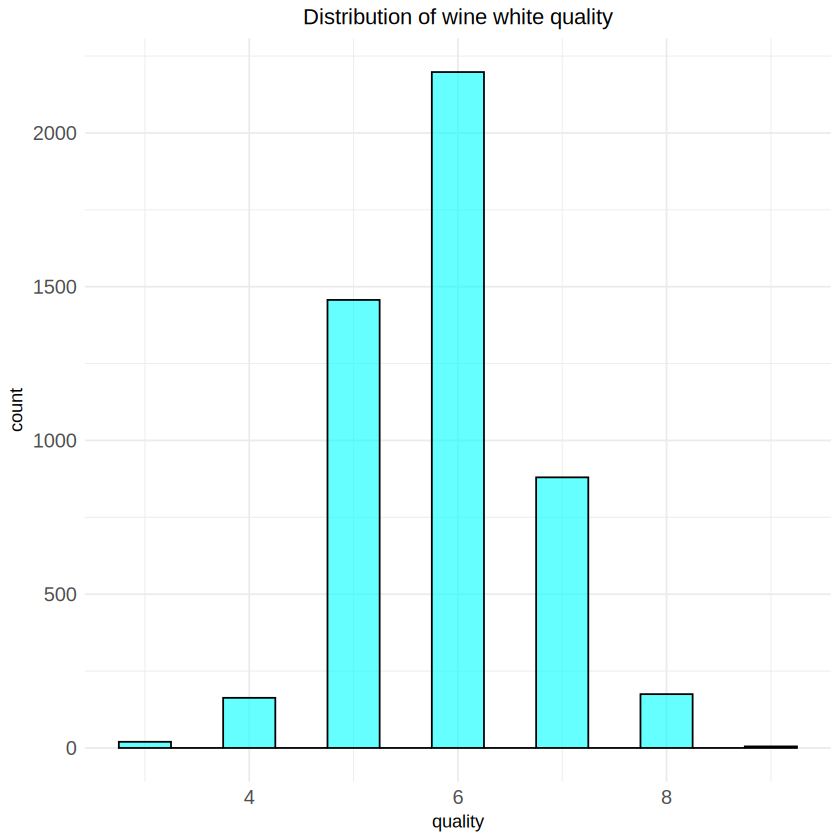
\includegraphics[width=0.75\columnwidth]{wine_figures/white_quality.png}
    \caption{Chất lượng rượu trắng.}
    \label{fig:white_quality}
\end{figure}
Nhận xét:
\begin{itemize}
    \item Chất lượng rượu có phân phối đối xứng 
    \item Hầu hết chất lượng rượu đỏ nằm ở mức 5, 6
    \item Không có rượu trắng nào đạt điểm tuyệt đối
    \item Chất lượng rượu trắng tệ nhất có điểm số là 3
\end{itemize}

% Khảo sát tính chua (acidity) trong rượu trắng
\textbf{Khảo sát tính chua (acidity) trong rượu trắng}
\begin{figure}[H]
    \centering
    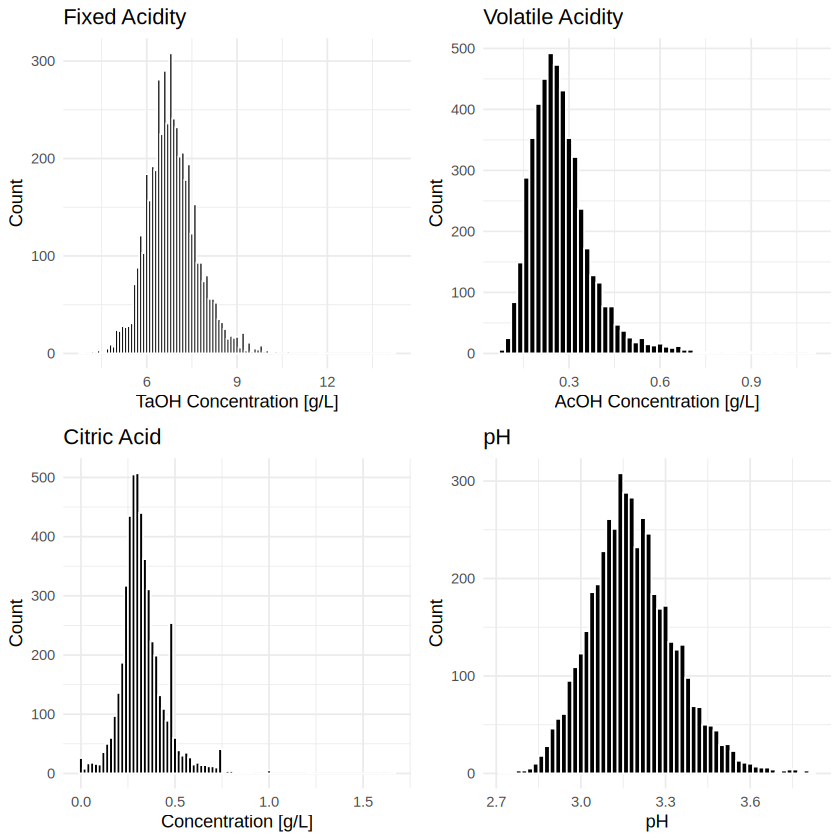
\includegraphics[width=0.75\columnwidth]{wine_figures/white_acidity.png}
    \caption{Histogram tính chua (acidity) trong rượu trắng.}
    \label{fig:white_acidity}
\end{figure}
Nhận xét:
\begin{itemize}
    \item Fixed và volatile acidity có phân phối (tương đối) bị lệch trái.
    \item Axit citric tạo thành phân bố biên vì một nhóm rượu vang dường như có nồng độ axit citric gần bằng 0.
    \item Histogram của pH tương đối đối xứng.
    \item Có một số ít các ngoại lại trong các biến này.
\end{itemize}

\begin{figure}[H]
    \centering
    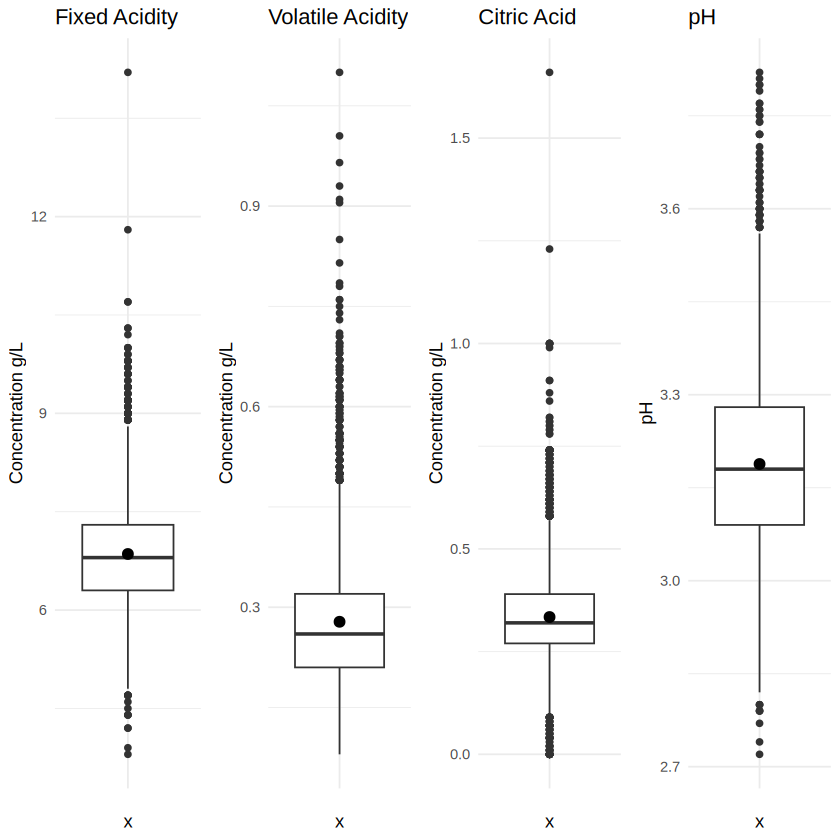
\includegraphics[width=0.75\columnwidth]{wine_figures/white_acidity_boxplot.png}
    \caption{Boxplot tính chua (acidity) trong rượu trắng.}
    \label{fig:white_acidity_boxplot}
\end{figure}
Nhận xét:
\begin{itemize}
    \item Nhìn vào các thông số độ axit trong biểu đồ hộp cho thấy một hình ảnh tương tự. 
    \item Ta có thể thấy đuôi dương dài của nồng độ axit cố định (fixed acide) và dễ bay hơi (volatile acide) và phân phối hẹp hơn đối với axit citric và độ pH. 
    \item Giá trị trung bình của axit citric và pH gần giá trị median hơn là giá trị trung bình của axit cố định (fixed acide) và dễ bay hơi (volatile acide).
\end{itemize}

% Khảo sát hàm lượng lưu huỳnh trong rượu trắng
\textbf{Khảo sát hàm lượng lưu huỳnh trong rượu trắng}
\begin{figure}[H]
    \centering
    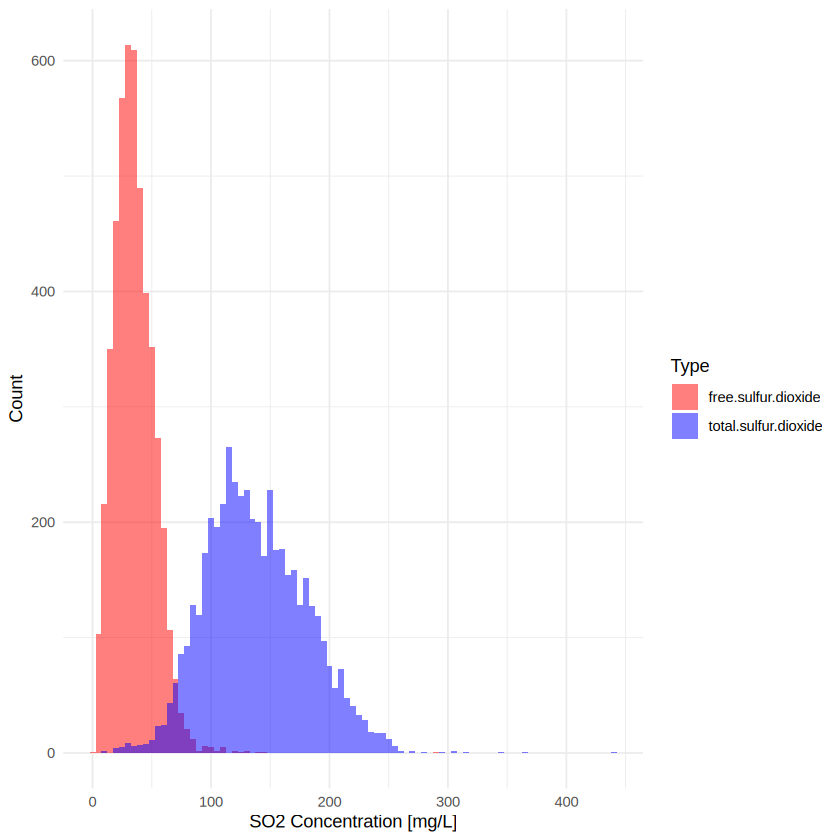
\includegraphics[width=0.75\columnwidth]{wine_figures/white_sulfur_dis.png}
    \caption{Phân phối SO2 tự do và tổng lượng SO2 trong rượu.}
    \label{fig:white_sulfur_dis}
\end{figure}
Nhận xét:
\begin{itemize}
    \item Nồng độ lưu huỳnh dioxit tự do tập trung hẹp quanh mức 50 mg/L. Nồng độ lưu huỳnh dioxit tổng thể cho thấy một phân phối tương đối đối xứng.
\end{itemize}

\begin{figure}[H]
    \centering
    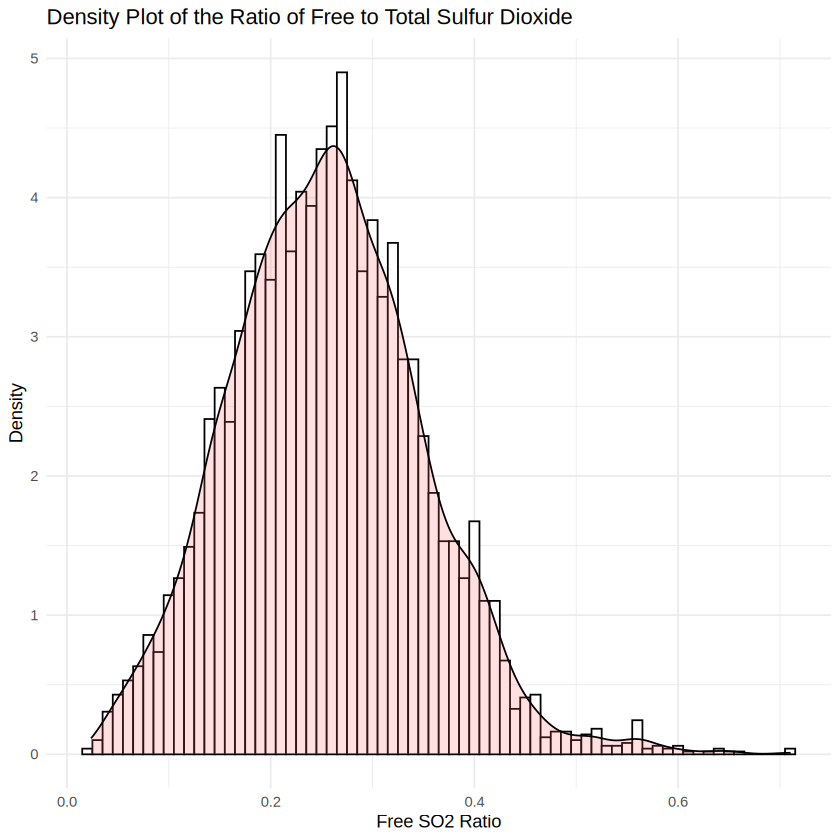
\includegraphics[width=0.75\columnwidth]{wine_figures/white_ratio.png}
    \caption{Phân phối tỷ lệ SO2 tự do và tổng lượng SO2.}
    \label{fig:white_free_so2}
\end{figure}
Nhận xét:
\begin{itemize}
    \item Khi vẽ biểu đồ tỷ lệ giữa lưu huỳnh dioxit tự do và lưu huỳnh dioxit tổng trong rượu vang, người ta có thể thấy rằng khoảng 30\% lưu huỳnh dioxit tổng xuất hiện ở dạng tự do. Sự phân bố bị lệch dương với một số loại rượu vang có tỷ lệ cao hơn đáng kể.
\end{itemize}

\begin{figure}[H]
    \centering
    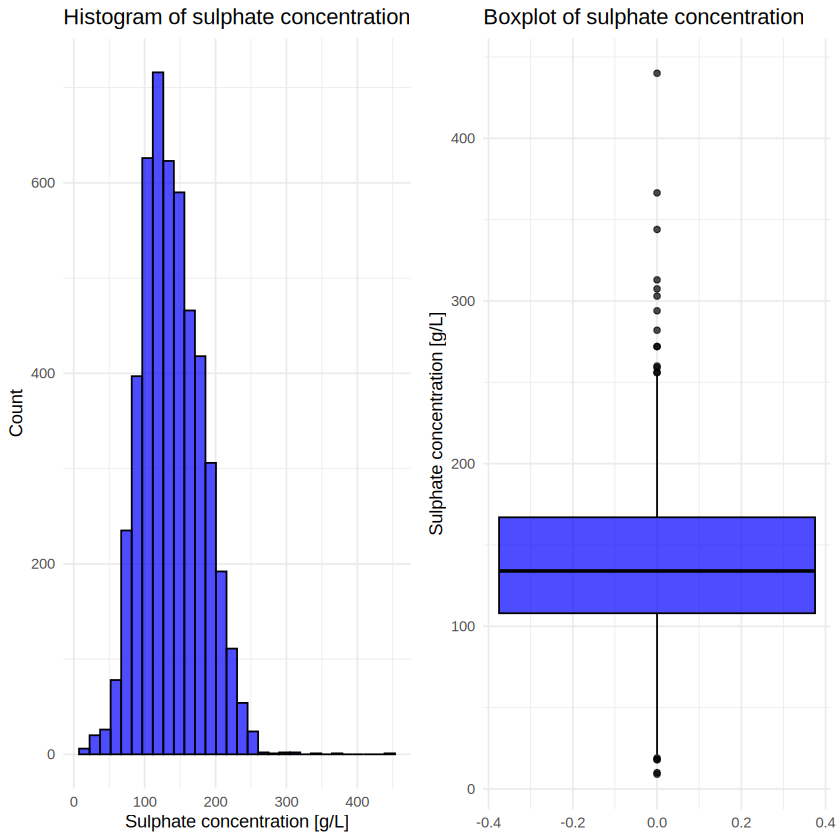
\includegraphics[width=0.75\columnwidth]{wine_figures/white_sulphate.png}
    \caption{Phân phối Lượng muối sunphat trong rượu.}
    \label{fig:white_sulphate}
\end{figure}
Nhận xét:
\begin{itemize}
    \item Hầu hết rượu vang trắng có nồng độ sulfat khoảng 0,5 g/L. Có thể thấy ba nhóm ngoại lệ nhỏ trong biểu đồ.
\end{itemize}

% Khảo sát lượng đường còn lại sau khi lên men trong rượu trắng
\textbf{Khảo sát lượng đường còn lại sau khi lên men trong rượu trắng}
\begin{figure}[H]
    \centering
    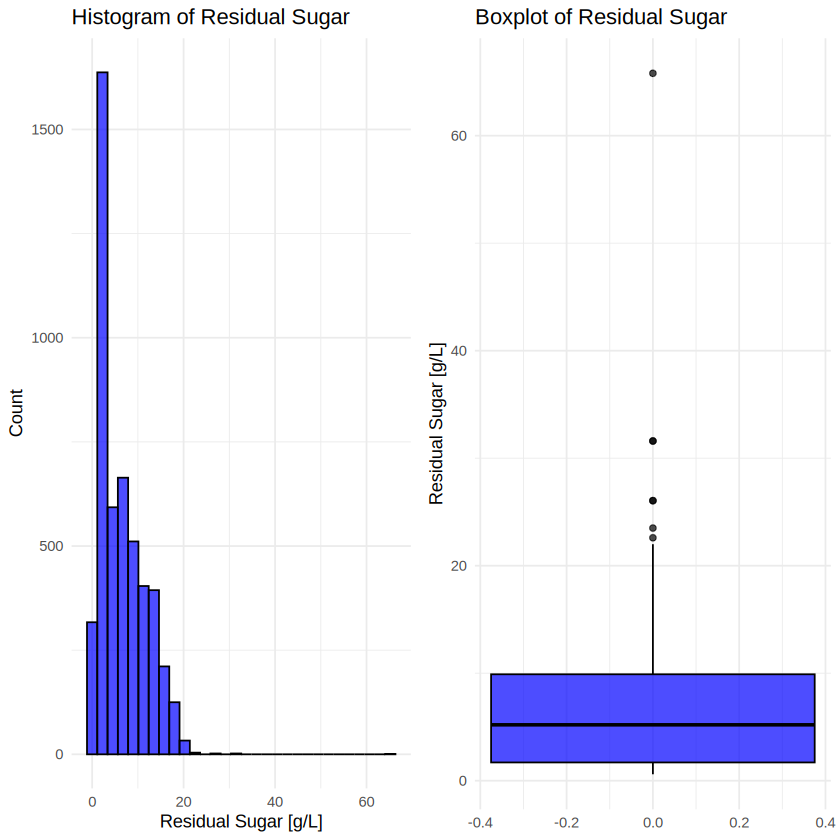
\includegraphics[width=0.75\columnwidth]{wine_figures/white_sugar.png}
    \caption{Phân phối lượng đường còn lại sau khi lên men trong rượu.}
    \label{fig:white_sugar}
\end{figure}
Nhận xét:
\begin{itemize}
    \item Nhìn chung, rượu vang trắng trong tập dữ liệu có vẻ có nồng độ đường dư thấp gần bằng 0. 
\end{itemize}

% Khảo sát phần trăm cồn trong rượu trắng
\textbf{Khảo sát phần trăm cồn trong rượu trắng}
\begin{figure}[H]
    \centering
    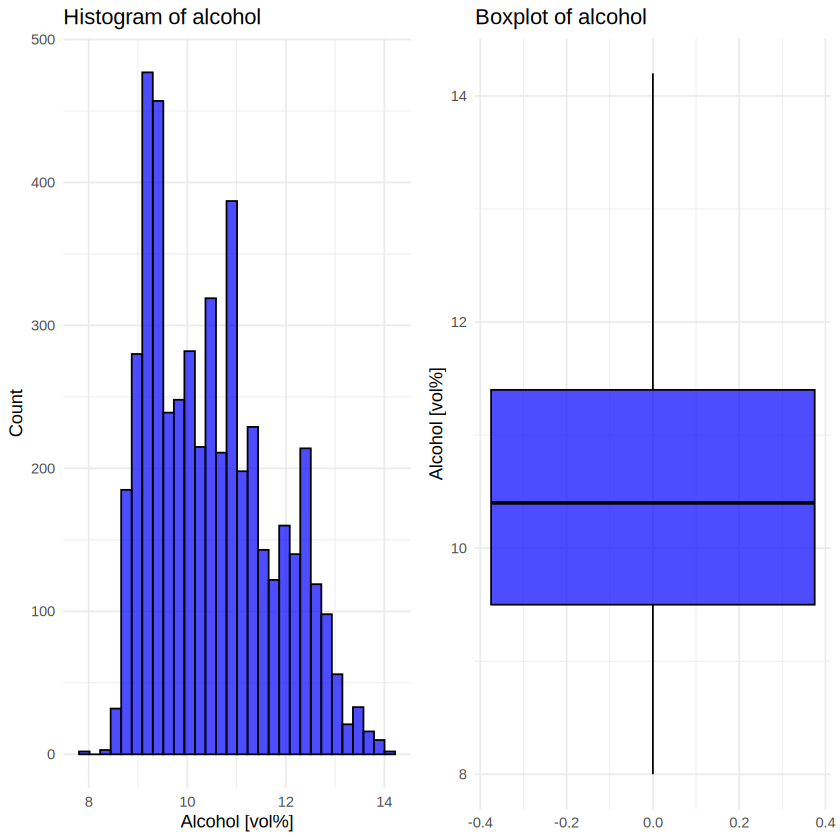
\includegraphics[width=0.75\columnwidth]{wine_figures/white_alcohol.png}
    \caption{Phân phối phần trăm cồn trong rượu.}
    \label{fig:white_alcohol}
\end{figure}
Nhận xét:
\begin{itemize}
    \item Hàm lượng cồn của rượu vang trong tập dữ liệu dao động từ 8 đến 15 vol\%. Giá trị trung bình nằm trong khoảng 10 vol. Phân phối khá rộng và cho thấy độ lệch dương.
\end{itemize}

% Khảo sát mật độ trong rượu trắng
\textbf{Khảo sát mật độ trong rượu trắng}
\begin{figure}[H]
    \centering
    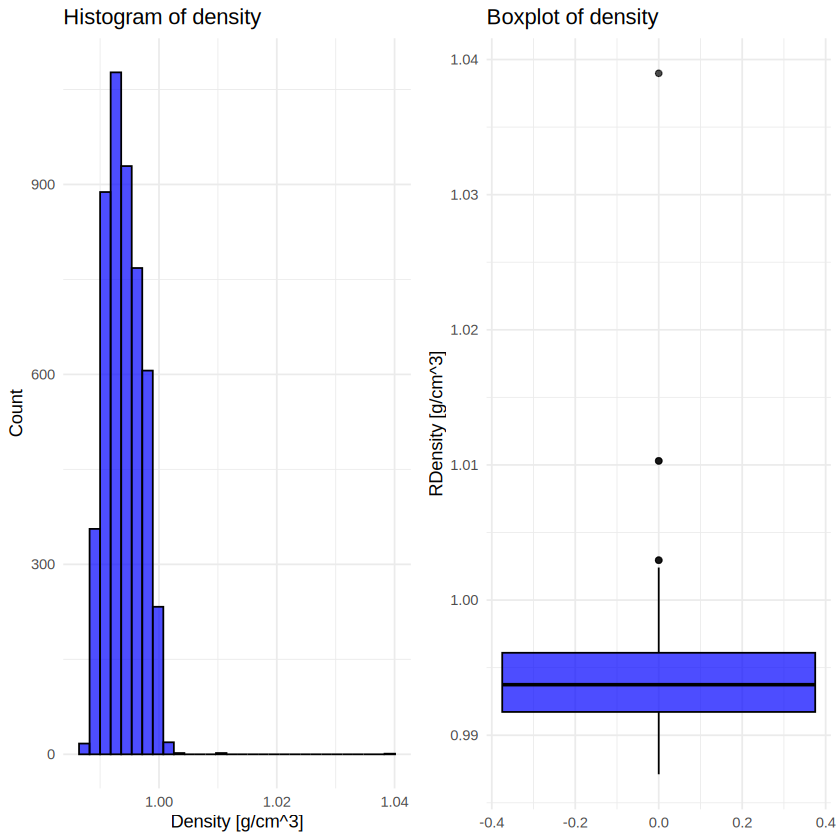
\includegraphics[width=0.75\columnwidth]{wine_figures/white_density.png}
    \caption{Phân phối mật độ rượu.}
    \label{fig:white_density}
\end{figure}
Nhận xét:
\begin{itemize}
    \item Tham số mật độ cho thấy sự phân bố rất hẹp với sự thay đổi thấp. Người ta có thể thấy một vài giá trị ngoại lệ trong khoảng 1,01 và 1,04 g/cm3 nhưng hầu hết các loại rượu vang có mật độ trong khoảng 0,99 và 1,00 g/cm3.
\end{itemize}

% Khảo sát lượng muối trong rượu trắng
\textbf{Khảo sát lượng muối trong rượu trắng}
\begin{figure}[H]
    \centering
    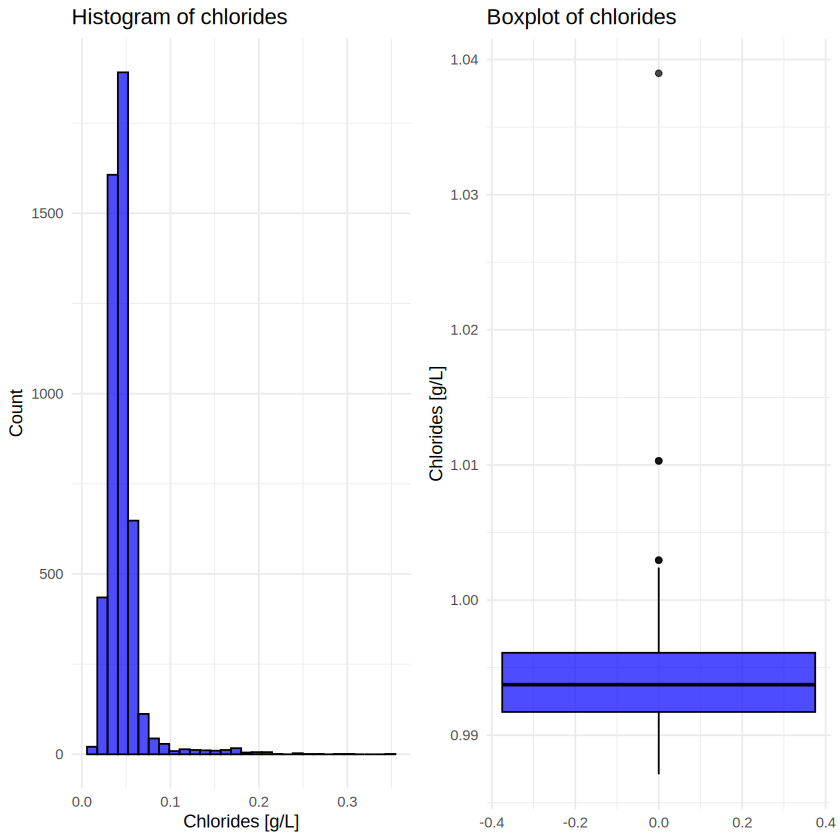
\includegraphics[width=0.75\columnwidth]{wine_figures/white_chlorides.png}
    \caption{Phân phối lượng muối rượu.}
    \label{fig:white_chlorides}
\end{figure}
Nhận xét:
\begin{itemize}
    \item Biểu đồ histogram của nồng độ clo cho thấy dữ liệu rượu trắng bị lệch.
\end{itemize}

\subsubsection{Phân tích đa biến}

\begin{figure}[H]
    \centering
    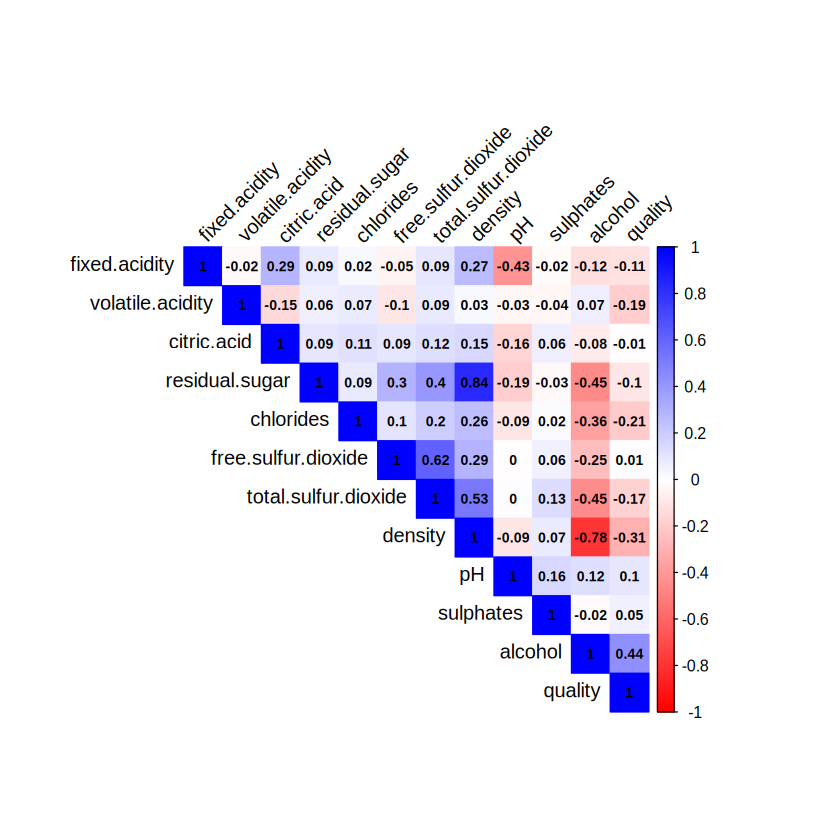
\includegraphics[width=0.75\columnwidth]{wine_figures/white_corr.png}
    \caption{Biểu đồ tương quan giữa các biến trong tập dữ liệu rượu trắng.}
    \label{fig:white_corr}
\end{figure}
Chọn ngưỡng là 0.3, ta thấy:
\begin{itemize}
    \item Nồng độ cồn (alcohol) có ảnh hưởng (thuận) đến chất lượng rượu (chỉ số tương quan 0.436)
    \item Các biến `residual.sugar` và `density` có tương quan thuận cao 0.83
\end{itemize}
Chọn ngưỡng là -0.3, ta thấy:
\begin{itemize}
    \item Mật độ trong rượu (`density`) có ảnh hưởng (nghịch) đến chất lượng của rượu (chỉ số tương quan -0.307)
    \item Các biến `alcohol` và `density` có tương quan nghịch cao -0.78
\end{itemize}

\subsubsection{Khảo sát đa cộng tuyến}

Bước 1: Tính toán chỉ số VIF
\begin{lstlisting}
fixed.acidity     volatile.acidity          citric.acid 
            2.691435             1.141156             1.165215 
      residual.sugar            chlorides  free.sulfur.dioxide 
           12.644064             1.236822             1.787880 
total.sulfur.dioxide              density                   pH 
            2.239233            28.232546             2.196362 
           sulphates              alcohol 
            1.138540             7.706957 
\end{lstlisting}
Nhận xét:
\begin{itemize}
    \item Ta có chọn ngưỡng bằng 3
\end{itemize}
Bước 2: Loại bỏ các biến dựa trên VIF nếu vượt quá ngưỡng
\begin{lstlisting}
fixed.acidity     volatile.acidity          citric.acid 
            1.356128             1.128298             1.159884 
      residual.sugar            chlorides  free.sulfur.dioxide 
            1.435215             1.203645             1.744627 
total.sulfur.dioxide                   pH            sulphates 
            2.153170             1.330912             1.056637 
             alcohol 
            1.647117 

Call:
lm(formula = quality ~ fixed.acidity + volatile.acidity + citric.acid + 
    residual.sugar + chlorides + free.sulfur.dioxide + total.sulfur.dioxide + 
    pH + sulphates + alcohol, data = wine_quality_white)

Residuals:
    Min      1Q  Median      3Q     Max 
-3.9098 -0.4957 -0.0330  0.4666  3.1785 

Coefficients:
                       Estimate Std. Error t value Pr(>|t|)    
(Intercept)           2.0636371  0.3482321   5.926 3.32e-09 ***
fixed.acidity        -0.0503197  0.0149092  -3.375 0.000744 ***
volatile.acidity     -1.9583442  0.1138553 -17.200  < 2e-16 ***
citric.acid          -0.0289483  0.0961455  -0.301 0.763360    
residual.sugar        0.0256438  0.0025518  10.049  < 2e-16 ***
chlorides            -0.9525303  0.5425208  -1.756 0.079194 .  
free.sulfur.dioxide   0.0047672  0.0008391   5.682 1.41e-08 ***
total.sulfur.dioxide -0.0008697  0.0003730  -2.331 0.019771 *  
pH                    0.1651688  0.0825418   2.001 0.045444 *  
sulphates             0.4193440  0.0973099   4.309 1.67e-05 ***
alcohol               0.3626941  0.0112672  32.190  < 2e-16 ***
---
Signif. codes:  0 '***' 0.001 '**' 0.01 '*' 0.05 '.' 0.1 ' ' 1

Residual standard error: 0.756 on 4887 degrees of freedom
Multiple R-squared:  0.2727,	Adjusted R-squared:  0.2713 
F-statistic: 183.3 on 10 and 4887 DF,  p-value: < 2.2e-16
\end{lstlisting}

\subsubsection{Khảo sát ngoại lai}

Ta sử dụng IQR để tìm các điểm ngoại lai và cực ngoại lai:
\begin{itemize}
    \item Tổng số ngoại lai: 1040
    \item Tổng số cực ngoại lai: 206
\end{itemize}
Trong bài toán này, ta sẽ loại bỏ các điểm cực ngoại lai

\subsubsection{Chuẩn hóa và phân chia tập dữ liệu}

Ta sử dụng box-cox tranform và sau đó phân chia tập dữ liệu thành 2 phần: train (80\%) và test (20\%).

\subsubsection{Mô hình hóa hồi quy tuyến tính đa biến}

\begin{lstlisting}
# Mô hình chặn dưới
model.lb <- lm(quality ~ 1, data = train)

# Mô hình chặn trên
model.up <- full.lm

step(full.lm, scope = list(lower = model.lb, upper = model.up), direction = "both", trace = FALSE)
\end{lstlisting}
Kết quả:
\begin{lstlisting}
lm(formula = quality ~ fixed.acidity + volatile.acidity + citric.acid + 
    residual.sugar + chlorides + free.sulfur.dioxide + total.sulfur.dioxide + 
    sulphates + alcohol, data = train)

Coefficients:
         (Intercept)         fixed.acidity      volatile.acidity  
          -1.812e+00            -1.266e-01            -1.267e-04  
         citric.acid        residual.sugar             chlorides  
           3.298e-03             4.790e-03            -8.670e-07  
 free.sulfur.dioxide  total.sulfur.dioxide             sulphates  
           2.258e-01             2.467e+00             2.396e-04  
             alcohol  
           2.036e+00  
\end{lstlisting}

\begin{lstlisting}
wqr_models <- regsubsets(quality ~ volatile.acidity + chlorides + density + pH + sulphates + alcohol, data = train)
summary.wqr <-summary(wqr_models)
\end{lstlisting}
Ta lựa chọn mô hình tốt nhất dựa trên BIC. Kết quả:
\begin{lstlisting}
lm(formula = as.formula(formula_str), data = train)

Residuals:
      Min        1Q    Median        3Q       Max 
-0.041608 -0.002218  0.000647  0.002862  0.024640 

Coefficients:
                      Estimate Std. Error t value Pr(>|t|)    
(Intercept)         -6.348e-01  4.355e-02 -14.576  < 2e-16 ***
fixed.acidity       -1.091e-01  2.976e-02  -3.667 0.000249 ***
volatile.acidity    -1.279e-04  1.118e-05 -11.432  < 2e-16 ***
residual.sugar       4.993e-03  5.319e-04   9.388  < 2e-16 ***
free.sulfur.dioxide  2.482e-01  1.874e-02  13.243  < 2e-16 ***
sulphates            2.405e-04  7.085e-05   3.394 0.000695 ***
alcohol              2.113e+00  7.701e-02  27.431  < 2e-16 ***
---
Signif. codes:  0 '***' 0.001 '**' 0.01 '*' 0.05 '.' 0.1 ' ' 1

Residual standard error: 0.004705 on 3746 degrees of freedom
Multiple R-squared:  0.2246,	Adjusted R-squared:  0.2234 
F-statistic: 180.8 on 6 and 3746 DF,  p-value: < 2.2e-16
\end{lstlisting}
Kiểm định phân phối chuẩn cho các giá trị thặng dư
\begin{itemize}
    \item H0: Biến thặng dư của mô hình phân phối chuẩn trong một số quần thể.
    \item H1: Biến thặng dư của mô hình không phân phối chuẩn trong một số quần thể.
\end{itemize}
\begin{figure}[H]
    \centering
    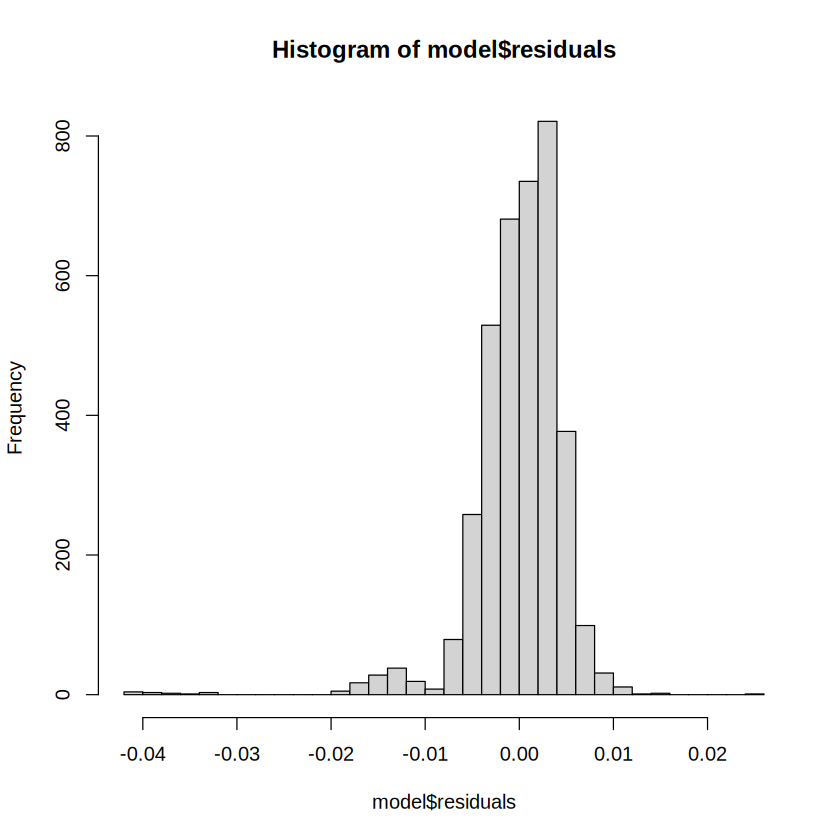
\includegraphics[width=0.75\columnwidth]{wine_figures/white_residual_test.png}
    \caption{Histogram của biến thặng dư mô hình.}
    \label{fig:white_residual_test}
\end{figure}
Kết quả:
\begin{lstlisting}
Shapiro-Wilk normality test

data:  model$residuals
W = 0.8476, p-value < 2.2e-16

[1] "H0 rejected: the residuals are NOT distributed normally"
\end{lstlisting}
Như vậy, biến thặng dư không có phân phối chuẩn. Như vậy, các phân tích về sau có thể chưa đủ độ tin cậy. Cần có những biến đổi để cải thiện kết quả phân tích.

Kiểm định phương sai đồng nhất bằng việc sử dụng Biểu đồ scale-location kiểm định giả định hồi quy về phương sai bằng nhau (homoscedasticity), tức là giá trị thặng dư có phương sai bằng với đường hồi quy.
\begin{itemize}
    \item H0: Các giá trị thặng dư là homoscedastic
    \item H1: Các giá trị thặng dư là heteroscedastic
\end{itemize}
\begin{figure}[H]
    \centering
    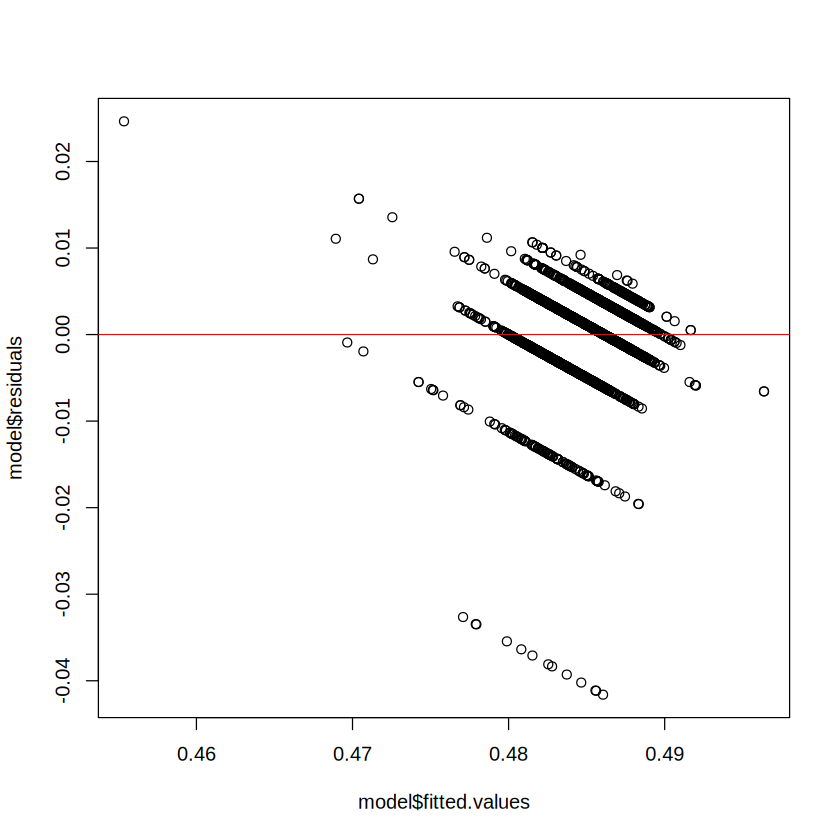
\includegraphics[width=0.75\columnwidth]{wine_figures/white_scale_test.png}
    \caption{Biểu đồ Heteroscedasticity.}
    \label{fig:white_scale_test}
\end{figure}
Kết quả:
\begin{lstlisting}
studentized Breusch-Pagan test

data:  model
BP = 140.19, df = 6, p-value < 2.2e-16

[1] "H0 rejected: Error variance spreads INCONSTANTLY/generating patterns (Heteroscedasticity)"(Heteroscedasticity)"
\end{lstlisting}
Như vậy, ta thấy p-value nhỏ hơn múc ý nghĩa 0.05, ta đủ điều kiện bác bỏ H0. Vậy các giá trị thặng dư là heteroscedastic.

\subsubsection{Kết quả dự đoán}

Dựa trên quá trình mô hình hóa, ta thu được mô hình

\begin{lstlisting}
quality = fixed.acidity + volatile.acidity + residual.sugar + free.sulfur.dioxide + sulphate + alcohol
\end{lstlisting}

với các hệ số:

\begin{lstlisting}
Coefficients:
(Intercept)        fixed.acidity     volatile.acidity  
         -0.6041273           -0.1045400           -0.0001204  
     residual.sugar  free.sulfur.dioxide            sulphates  
          0.0039231            0.2933424            0.0001746  
            alcohol  
          2.0023690 
\end{lstlisting}

Điều này có nghĩa là:
\begin{itemize}
    \item Chất lượng rượu phụ thuộc vào nồng độ cồn, nồng độ cồn càng cao, chất lượng rượu càng tăng.
    \item Các chỉ số về tính chua khiến chất lượng của rượu bị giảm.
    \item  Lượng đường, muối nhỏ có thể giúp rượu trắng ngon hơn.
    \item Khí SO2 có tác động tích cực đến chất lượng rượu trắng
\end{itemize}


\subsection{Phân tích chất lượng rượu đỏ}

\subsubsection{Các thông tin thống kê mô tả về bộ dữ liệu}

\begin{lstlisting}
   variable             missing   min lower median upper     max
   <chr>                  <dbl> <dbl> <dbl>  <dbl> <dbl>   <dbl>
 1 fixed.acidity              0 4.6     7.1    7.9   9.2  15.9  
 2 volatile.acidity           0 0.12    0.4    0.5   0.6   1.58 
 3 citric.acid                0 0       0.1    0.3   0.4   1    
 4 residual.sugar             0 0.9     1.9    2.2   2.6  15.5  
 5 chlorides                  0 0.012   0.1    0.1   0.1   0.611
 6 free.sulfur.dioxide        0 1       7     14    21    72    
 7 total.sulfur.dioxide       0 6      22     38    62   289    
 8 density                    0 0.990   1      1     1     1.00 
 9 pH                         0 2.74    3.2    3.3   3.4   4.01 
10 sulphates                  0 0.33    0.6    0.6   0.7   2    
11 alcohol                    0 8.4     9.5   10.2  11.1  14.9  
12 quality                    0 3       5      6     6     8   
\end{lstlisting}
Nhận xét:
\begin{itemize}
    \item 
\end{itemize}

\subsubsection{Phân tích đơn biến}

% Chất lượng rượu
\textbf{Chất lượng rượu đỏ}
\begin{figure}[H]
    \centering
    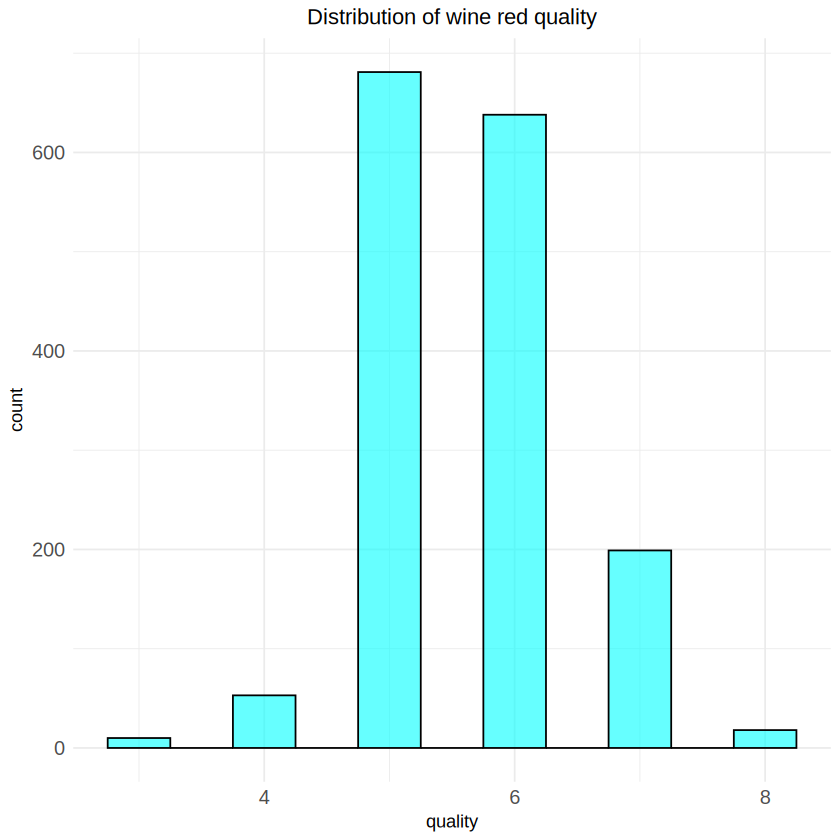
\includegraphics[width=0.75\columnwidth]{wine_figures/red_quality.png}
    \caption{Chất lượng rượu đỏ.}
    \label{fig:red_quality}
\end{figure}
Nhận xét:
\begin{itemize}
    \item Chất lượng rượu có phân phối đối xứng 
    \item Hầu hết chất lượng rượu đỏ nằm ở mức 5, 6
    \item Không có rượu đỏ nào đạt điểm tuyệt đối
    \item Chất lượng rượu đỏ tệ nhất có điểm số là 3
\end{itemize}

% Khảo sát tính chua (acidity) trong rượu đỏ
\textbf{Khảo sát tính chua (acidity) trong rượu đỏ}
\begin{figure}[H]
    \centering
    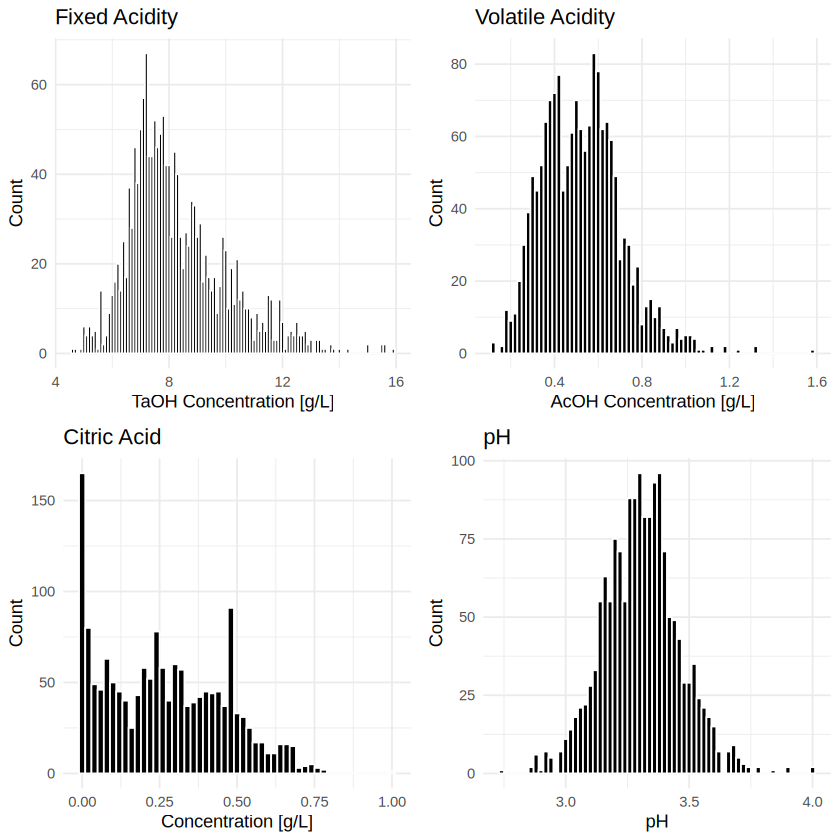
\includegraphics[width=0.75\columnwidth]{wine_figures/red_acidity.png}
    \caption{Histogram tính chua (acidity) trong rượu đỏ.}
    \label{fig:red_acidity}
\end{figure}
Nhận xét:
\begin{itemize}
    \item Fixed và volatile acidity có phân phối (tương đối) bị lệch trái.
    \item Axit citric tạo thành phân bố biên vì một nhóm rượu vang dường như có nồng độ axit citric gần bằng 0.
    \item Histogram của pH tương đối đối xứng.
    \item Có một số ít các ngoại lại trong các biến này.
\end{itemize}

\begin{figure}[H]
    \centering
    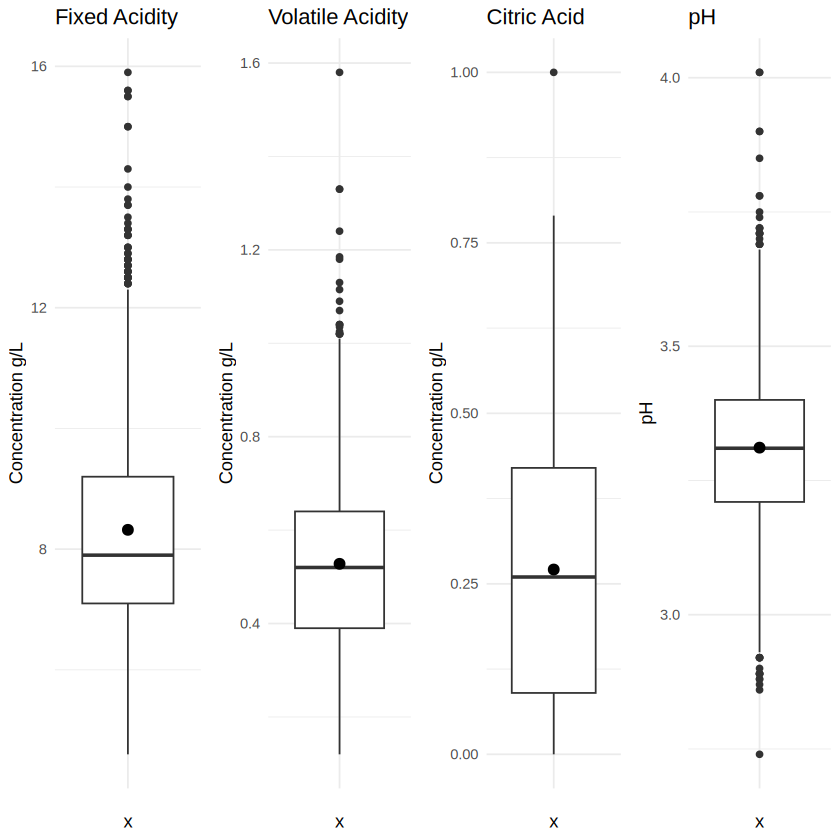
\includegraphics[width=0.75\columnwidth]{wine_figures/red_acidity_boxplot.png}
    \caption{Boxplot tính chua (acidity) trong rượu đỏ.}
    \label{fig:red_acidity_boxplot}
\end{figure}
Nhận xét:
\begin{itemize}
    \item Nhìn vào các thông số độ axit trong biểu đồ hộp cho thấy một hình ảnh tương tự. 
    \item Ta có thể thấy đuôi dương dài của nồng độ axit cố định (fixed acide) và dễ bay hơi (volatile acide) và phân phối hẹp hơn đối với axit citric và độ pH. 
    \item Giá trị trung bình của axit citric và pH gần giá trị median hơn là giá trị trung bình của axit cố định (fixed acide) và dễ bay hơi (volatile acide).
\end{itemize}

% Khảo sát hàm lượng lưu huỳnh trong rượu đỏ
\textbf{Khảo sát hàm lượng lưu huỳnh trong rượu đỏ}
\begin{figure}[H]
    \centering
    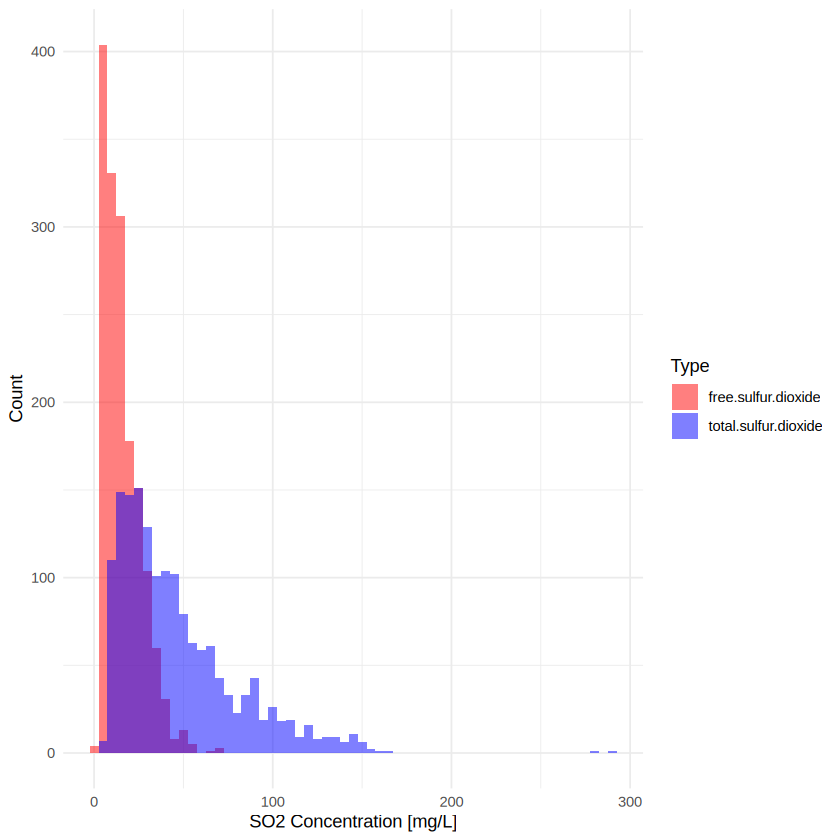
\includegraphics[width=0.75\columnwidth]{wine_figures/red_sulfur_dis.png}
    \caption{Phân phối SO2 tự do và tổng lượng SO2 trong rượu.}
    \label{fig:red_sulfur_dis}
\end{figure}
Nhận xét:
\begin{itemize}
    \item Nồng độ lưu huỳnh dioxit tự do tập trung hẹp quanh mức 30 mg/L. Nồng độ lưu huỳnh dioxit tổng thể cho thấy một phân phối bị lệch trái.
\end{itemize}

\begin{figure}[H]
    \centering
    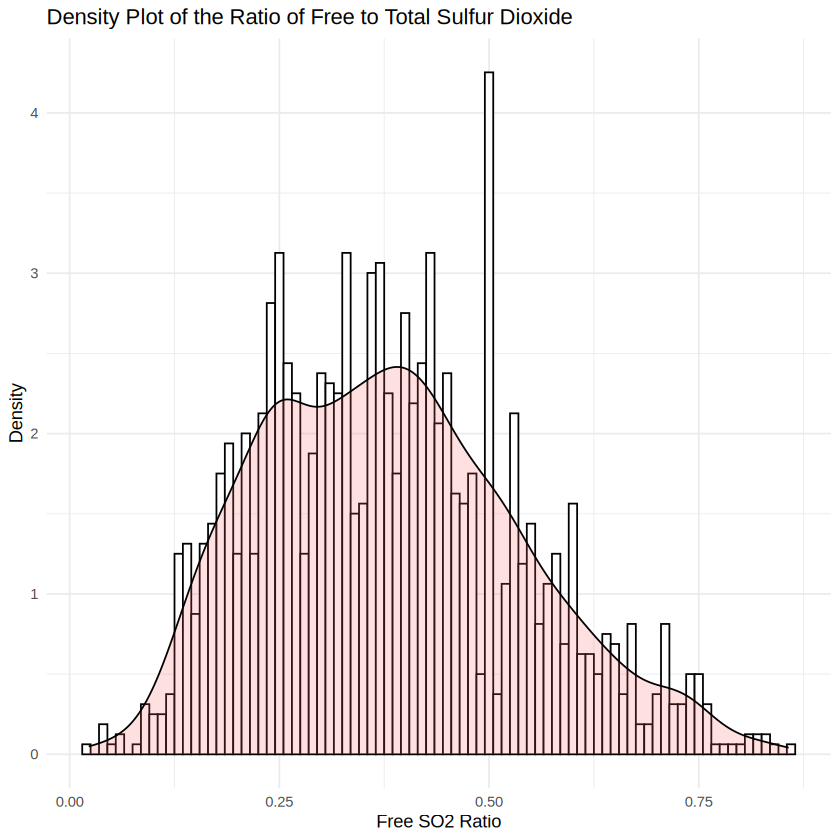
\includegraphics[width=0.75\columnwidth]{wine_figures/red_ratio.png}
    \caption{Phân phối tỷ lệ SO2 tự do và tổng lượng SO2.}
    \label{fig:red_free_so2}
\end{figure}
Nhận xét:
\begin{itemize}
    \item Khi vẽ biểu đồ tỷ lệ giữa lưu huỳnh dioxit tự do và lưu huỳnh dioxit tổng trong rượu vang, người ta có thể thấy rằng khoảng 30\% lưu huỳnh dioxit tổng xuất hiện ở dạng tự do. Sự phân bố bị lệch dương với một số loại rượu vang có tỷ lệ cao hơn đáng kể. Điểm đáng chú ý nữa là đỉnh xuất hiện chính xác ở mức 0,5.
\end{itemize}

\begin{figure}[H]
    \centering
    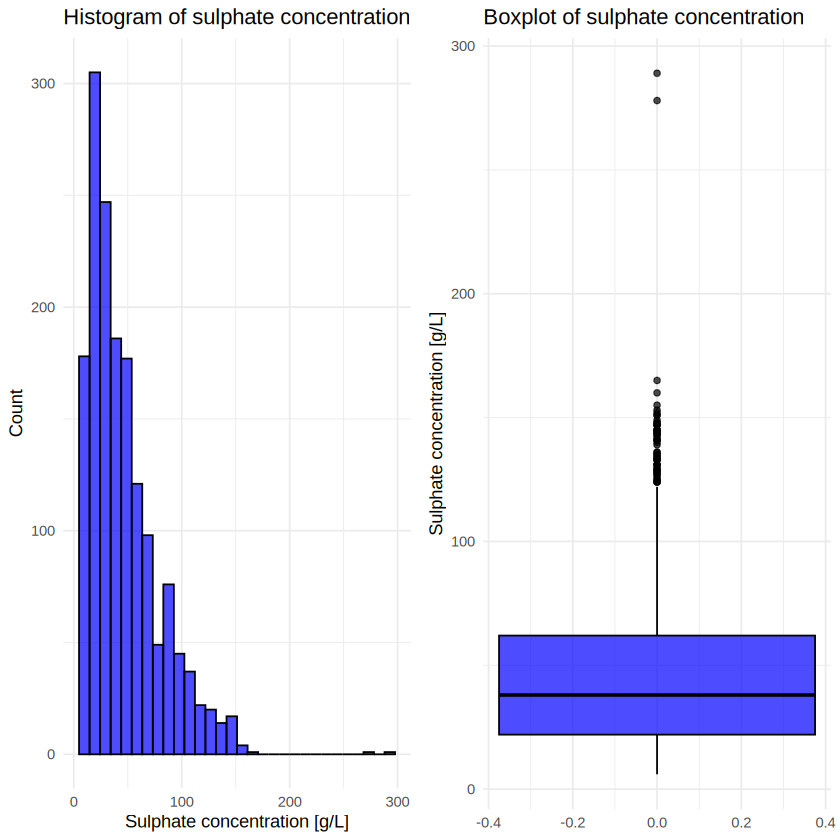
\includegraphics[width=0.75\columnwidth]{wine_figures/red_sulphate.png}
    \caption{Phân phối Lượng muối sunphat trong rượu.}
    \label{fig:red_sulphate}
\end{figure}
Nhận xét:
\begin{itemize}
    \item Hầu hết rượu vang đỏ có nồng độ sulfat khoảng 0,5 g/L. Có thể thấy ba nhóm ngoại lệ nhỏ trong biểu đồ.
\end{itemize}

% Khảo sát lượng đường còn lại sau khi lên men trong rượu đỏ
\textbf{Khảo sát lượng đường còn lại sau khi lên men trong rượu đỏ}
\begin{figure}[H]
    \centering
    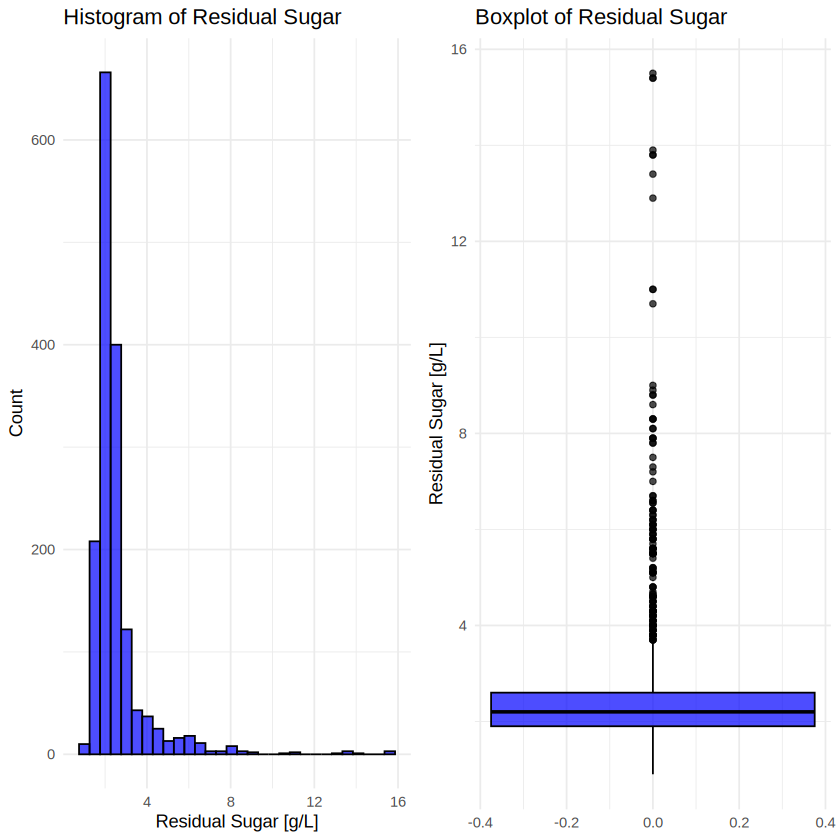
\includegraphics[width=0.75\columnwidth]{wine_figures/red_sugar.png}
    \caption{Phân phối lượng đường còn lại sau khi lên men trong rượu.}
    \label{fig:red_sugar}
\end{figure}
Nhận xét:
\begin{itemize}
    \item Nhìn chung, rượu vang đỏ trong tập dữ liệu có vẻ có nồng độ đường dư thấp gần bằng 0. 
\end{itemize}

% Khảo sát phần trăm cồn trong rượu đỏ
\textbf{Khảo sát phần trăm cồn trong rượu đỏ}
\begin{figure}[H]
    \centering
    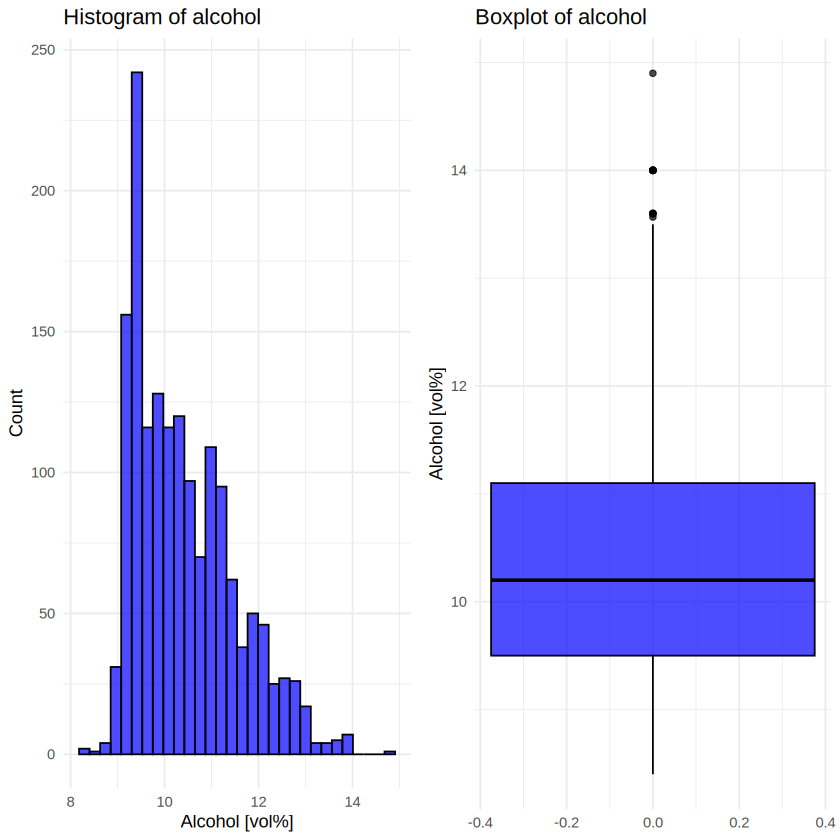
\includegraphics[width=0.75\columnwidth]{wine_figures/red_alcohol.png}
    \caption{Phân phối phần trăm cồn trong rượu.}
    \label{fig:red_alcohol}
\end{figure}
Nhận xét:
\begin{itemize}
    \item Hàm lượng cồn của rượu vang đỏ trong tập dữ liệu dao động từ 8 đến 15 vol\%. Giá trị trung bình nằm trong khoảng 10 vol. Phân phối khá rộng và cho thấy độ lệch dương.
\end{itemize}

% Khảo sát mật độ trong rượu đỏ
\textbf{Khảo sát mật độ trong rượu đỏ}
\begin{figure}[H]
    \centering
    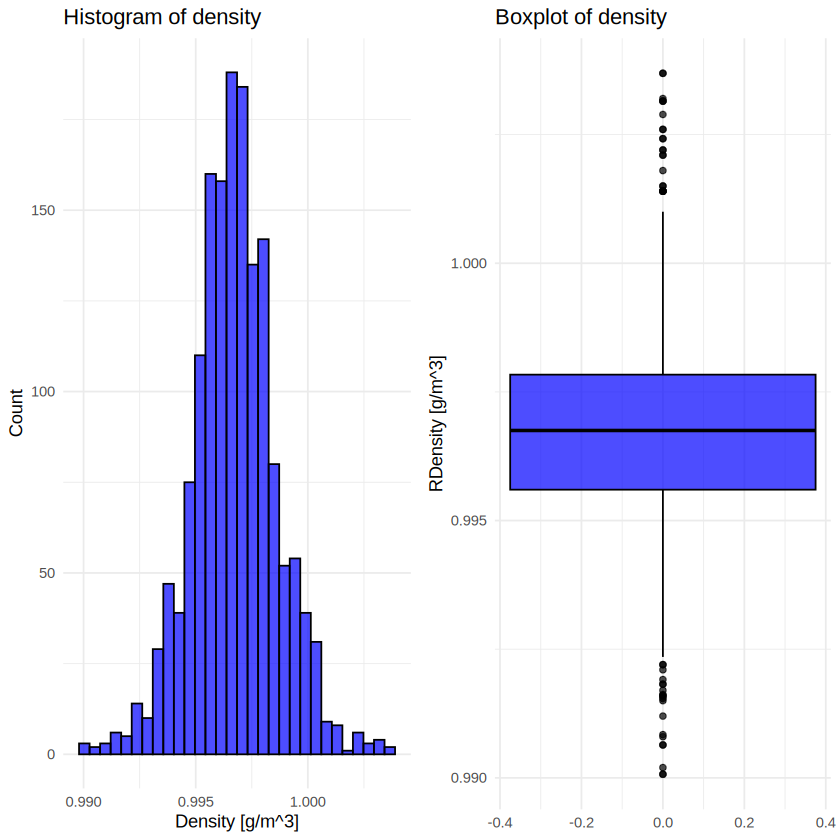
\includegraphics[width=0.75\columnwidth]{wine_figures/red_density.png}
    \caption{Phân phối mật độ rượu.}
    \label{fig:red_density}
\end{figure}
Nhận xét:
\begin{itemize}
    \item Tham số mật độ cho thấy sự phân bố rất hẹp với sự thay đổi thấp. Người ta có thể thấy một vài giá trị ngoại lệ trong khoảng 1,01 và 1,04 g/cm3 nhưng hầu hết các loại rượu vang có mật độ trong khoảng 0,99 và 1,00 g/cm3.
\end{itemize}

% Khảo sát lượng muối trong rượu đỏ
\textbf{Khảo sát lượng muối trong rượu đỏ}
\begin{figure}[H]
    \centering
    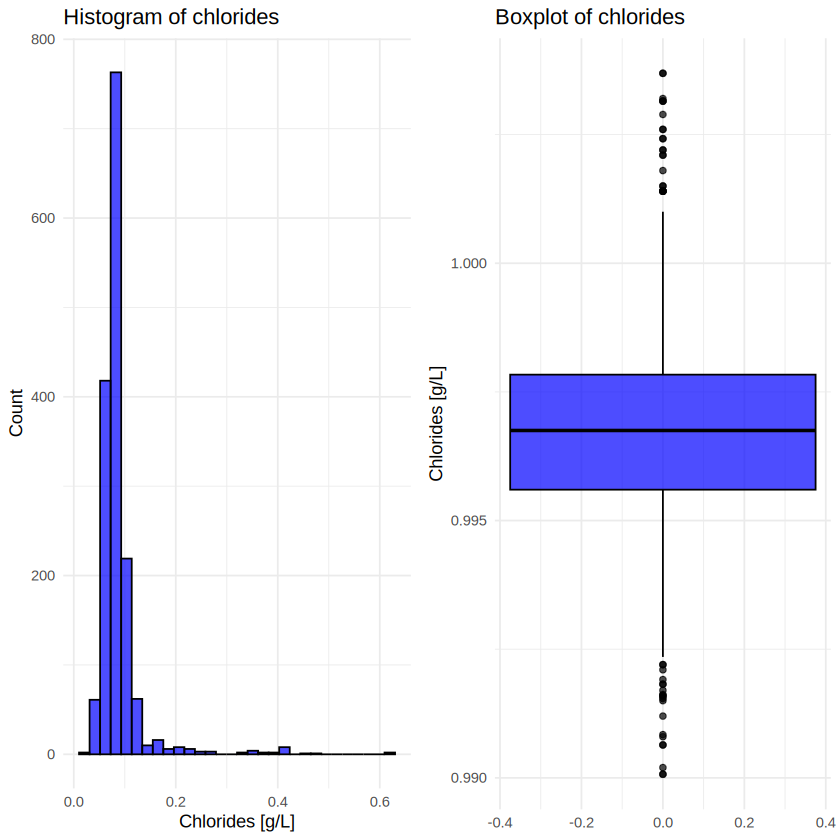
\includegraphics[width=0.75\columnwidth]{wine_figures/red_chlorides.png}
    \caption{Phân phối lượng muối rượu.}
    \label{fig:red_chlorides}
\end{figure}
Nhận xét:
\begin{itemize}
    \item Biểu đồ histogram của nồng độ clo cho thấy dữ liệu rượu đỏ tương dối cân bằng.
\end{itemize}

\subsubsection{Phân tích đa biến}

\begin{figure}[H]
    \centering
    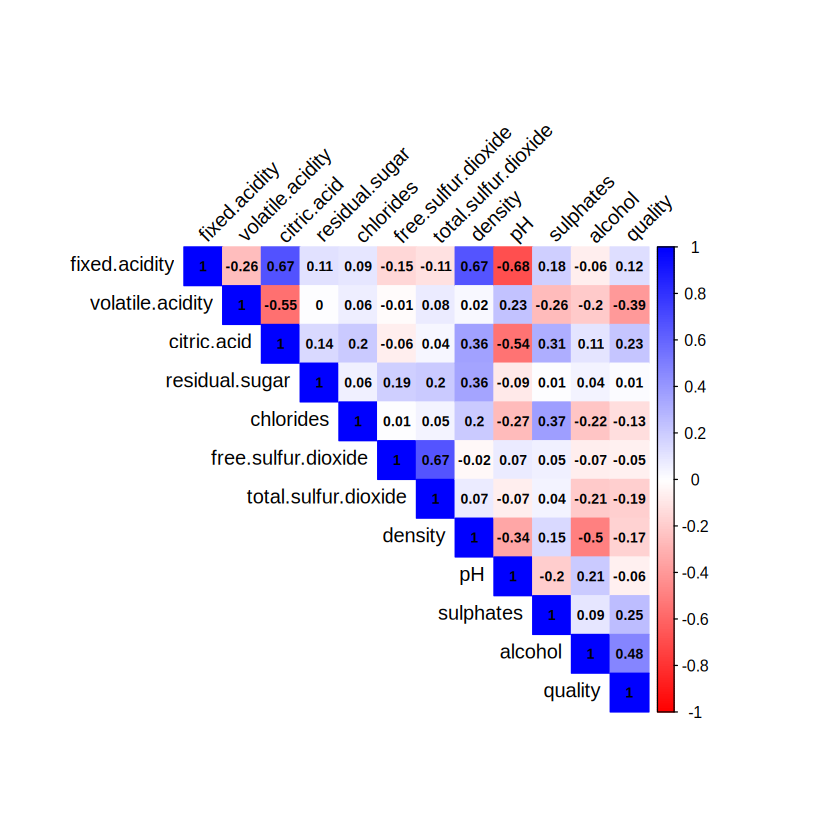
\includegraphics[width=0.75\columnwidth]{wine_figures/red_corr.png}
    \caption{Biểu đồ tương quan giữa các biến trong tập dữ liệu rượu đỏ.}
    \label{fig:red_corr}
\end{figure}
Chọn ngưỡng là 0.3, ta thấy:
\begin{itemize}
    \item Nồng độ cồn (alcohol) có ảnh hưởng (thuận) đến chất lượng rượu (chỉ số tương quan 0.476)
    \item Các biến `residual.sugar` và `density` có tương quan thuận thấp 0.35
    \item Biến fixed.acidity và citric.acid có tương quan dương mạnh, 0.671
\end{itemize}
Chọn ngưỡng là -0.3, ta thấy:
\begin{itemize}
    \item Mật độ trong rượu (`density`) có ảnh hưởng (nghịch) đến pH của rượu (chỉ số tương quan -0.34) và alcohol (-0.496)
\end{itemize}


\subsubsection{Khảo sát đa cộng tuyến}

Bước 1: Tính toán chỉ số VIF
\begin{lstlisting}
fixed.acidity     volatile.acidity          citric.acid 
            7.767512             1.789390             3.128022 
      residual.sugar            chlorides  free.sulfur.dioxide 
            1.702588             1.481932             1.963019 
total.sulfur.dioxide              density                   pH 
            2.186813             6.343760             3.329732 
           sulphates              alcohol 
            1.429434             3.031160 
\end{lstlisting}
Nhận xét:
\begin{itemize}
    \item Ta có chọn ngưỡng bằng 3
\end{itemize}
Bước 2: Loại bỏ các biến dựa trên VIF nếu vượt quá ngưỡng
\begin{lstlisting}
 volatile.acidity          citric.acid       residual.sugar 
            1.784963             2.780557             1.386375 
           chlorides  free.sulfur.dioxide total.sulfur.dioxide 
            1.401232             1.939209             2.069396 
             density                   pH            sulphates 
            2.430096             1.610775             1.396382 
             alcohol 
            2.136067 

Call:
lm(formula = quality ~ volatile.acidity + citric.acid + residual.sugar + 
    chlorides + free.sulfur.dioxide + total.sulfur.dioxide + 
    density + pH + sulphates + alcohol, data = wine_quality_red)

Residuals:
     Min       1Q   Median       3Q      Max 
-2.65461 -0.36856 -0.04552  0.45670  2.03464 

Coefficients:
                       Estimate Std. Error t value Pr(>|t|)    
(Intercept)           6.1795700 13.4367180   0.460   0.6456    
volatile.acidity     -1.0777894  0.1209486  -8.911  < 2e-16 ***
citric.acid          -0.1353226  0.1387582  -0.975   0.3296    
residual.sugar        0.0101047  0.0135372   0.746   0.4555    
chlorides            -1.9684566  0.4076978  -4.828 1.51e-06 ***
free.sulfur.dioxide   0.0045916  0.0021580   2.128   0.0335 *  
total.sulfur.dioxide -0.0034272  0.0007089  -4.835 1.46e-06 ***
density              -1.5167406 13.3889717  -0.113   0.9098    
pH                   -0.5462340  0.1332577  -4.099 4.36e-05 ***
sulphates             0.8995900  0.1130053   7.961 3.23e-15 ***
alcohol               0.2900579  0.0222316  13.047  < 2e-16 ***
---
Signif. codes:  0 '***' 0.001 '**' 0.01 '*' 0.05 '.' 0.1 ' ' 1

Residual standard error: 0.648 on 1588 degrees of freedom
Multiple R-squared:  0.3602,	Adjusted R-squared:  0.3561 
F-statistic: 89.39 on 10 and 1588 DF,  p-value: < 2.2e-16
\end{lstlisting}


\subsubsection{Khảo sát ngoại lai}

Ta sử dụng IQR để tìm các điểm ngoại lai và cực ngoại lai:
\begin{itemize}
    \item Tổng số ngoại lai: 393
    \item Tổng số cực ngoại lai: 160
\end{itemize}
Trong bài toán này, ta sẽ loại bỏ các điểm cực ngoại lai

\subsubsection{Chuẩn hóa và phân chia tập dữ liệu}

Ta sử dụng box-cox tranform và sau đó phân chia tập dữ liệu thành 2 phần: train (80\%) và test (20\%).

\subsubsection{Mô hình hóa hồi quy tuyến tính đa biến}

\begin{lstlisting}
# Mô hình chặn dưới
model.lb <- lm(quality ~ 1, data = train)

# Mô hình chặn trên
model.up <- full.lm

step(full.lm, scope = list(lower = model.lb, upper = model.up), direction = "both", trace = FALSE)
\end{lstlisting}
Kết quả:
\begin{lstlisting}
lm(formula = quality ~ volatile.acidity + chlorides + density + 
    pH + sulphates + alcohol, data = train)

Coefficients:
     (Intercept)  volatile.acidity         chlorides           density  
      -2.489e-01        -2.356e-04        -2.089e-06        -2.798e-01  
              pH         sulphates           alcohol  
      -1.626e-01         2.639e-03         1.629e+00 
\end{lstlisting}

\begin{lstlisting}
wqr_models <- regsubsets(quality ~ volatile.acidity + chlorides + density + pH + sulphates + alcohol, data = train)
summary.wqr <-summary(wqr_models)
\end{lstlisting}
Ta lựa chọn mô hình tốt nhất dựa trên BIC. Kết quả:
\begin{lstlisting}
lm(formula = as.formula(formula_str), data = train)

Residuals:
      Min        1Q    Median        3Q       Max 
-0.039242 -0.001816  0.000235  0.002780  0.009180 

Coefficients:
                   Estimate Std. Error t value Pr(>|t|)    
(Intercept)      -2.579e-01  8.929e-02  -2.888 0.003952 ** 
volatile.acidity -2.447e-04  4.915e-05  -4.979 7.38e-07 ***
density          -3.156e-01  8.656e-02  -3.646 0.000279 ***
pH               -1.648e-01  3.290e-02  -5.008 6.36e-07 ***
sulphates         2.545e-03  2.811e-04   9.054  < 2e-16 ***
alcohol           1.649e+00  1.773e-01   9.300  < 2e-16 ***
---
Signif. codes:  0 '***' 0.001 '**' 0.01 '*' 0.05 '.' 0.1 ' ' 1

Residual standard error: 0.004389 on 1145 degrees of freedom
Multiple R-squared:  0.2724,	Adjusted R-squared:  0.2693 
F-statistic: 85.75 on 5 and 1145 DF,  p-value: < 2.2e-16
\end{lstlisting}
Kiểm định phân phối chuẩn cho các giá trị thặng dư
\begin{itemize}
    \item H0: Biến thặng dư của mô hình phân phối chuẩn trong một số quần thể.
    \item H1: Biến thặng dư của mô hình không phân phối chuẩn trong một số quần thể.
\end{itemize}
\begin{figure}[H]
    \centering
    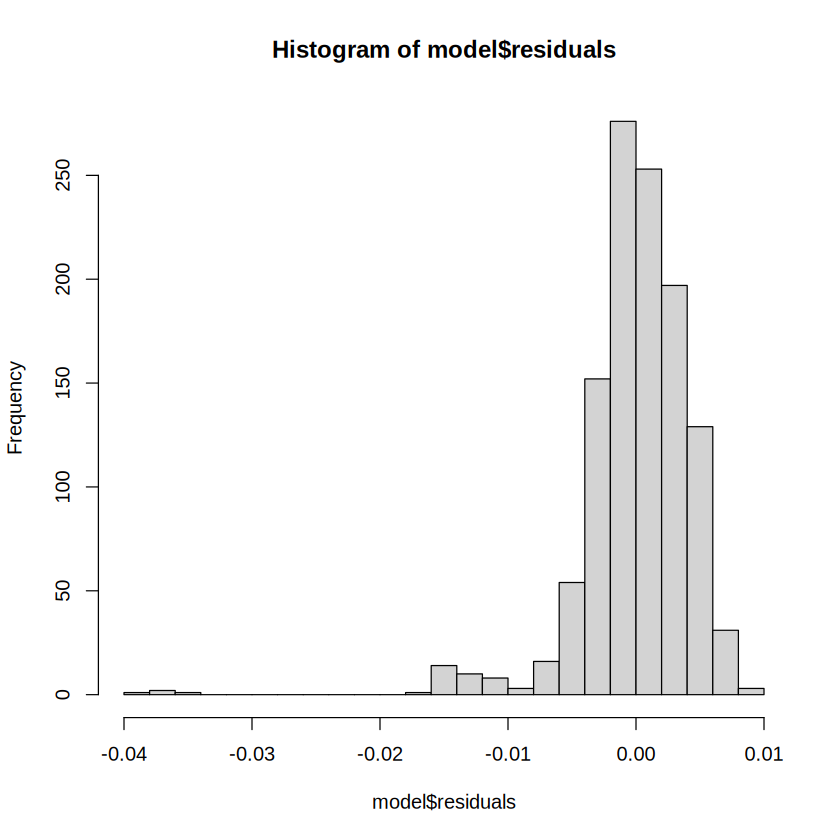
\includegraphics[width=0.75\columnwidth]{wine_figures/red_residual_test.png}
    \caption{Histogram của biến thặng dư mô hình.}
    \label{fig:red_residual_test}
\end{figure}
Kết quả:
\begin{lstlisting}
Shapiro-Wilk normality test

data:  model$residuals
W = 0.81862, p-value < 2.2e-16

[1] "H0 rejected: the residuals are NOT distributed normally"
\end{lstlisting}
Như vậy, biến thặng dư không có phân phối chuẩn. Như vậy, các phân tích về sau có thể chưa đủ độ tin cậy. Cần có những biến đổi để cải thiện kết quả phân tích.

Kiểm định phương sai đồng nhất bằng việc sử dụng Biểu đồ scale-location kiểm định giả định hồi quy về phương sai bằng nhau (homoscedasticity), tức là giá trị thặng dư có phương sai bằng với đường hồi quy.
\begin{itemize}
    \item H0: Các giá trị thặng dư là homoscedastic
    \item H1: Các giá trị thặng dư là heteroscedastic
\end{itemize}
\begin{figure}[H]
    \centering
    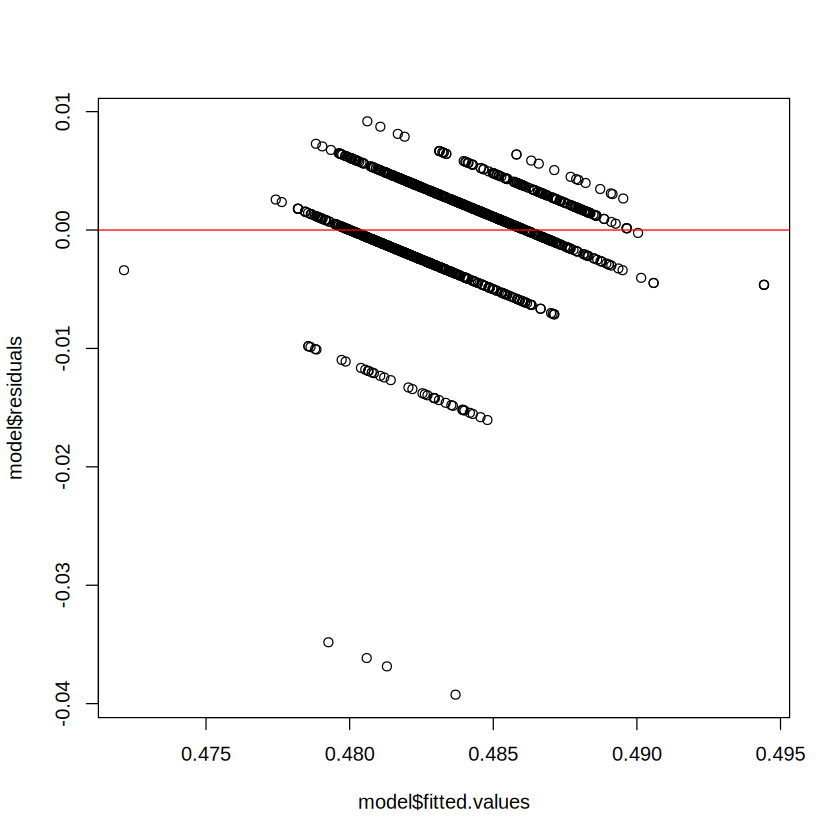
\includegraphics[width=0.75\columnwidth]{wine_figures/red_scale_test.png}
    \caption{Biểu đồ Heteroscedasticity.}
    \label{fig:red_scale_test}
\end{figure}
Kết quả:
\begin{lstlisting}
studentized Breusch-Pagan test

data:  model
BP = 15.396, df = 5, p-value = 0.008798

[1] "H0 rejected: Error variance spreads INCONSTANTLY/generating patterns (Heteroscedasticity)"
\end{lstlisting}
Như vậy, ta thấy p-value nhỏ hơn múc ý nghĩa 0.05, ta đủ điều kiện bác bỏ H0. Vậy các giá trị thặng dư là heteroscedastic

\subsubsection{Kết quả dự đoán}

Dựa trên quá trình mô hình hóa, ta thu được mô hình

\begin{lstlisting}
quality = volatile.acidity + density + pH + sulphates + alcohol
\end{lstlisting}

với các hệ số:
\begin{lstlisting}
Coefficients:
     (Intercept)  volatile.acidity           density                pH  
      -0.3675126        -0.0002588        -0.1598464        -0.0902720  
       sulphates           alcohol  
       0.0021522         1.8035125 
\end{lstlisting}

Điều này có nghĩa là:
\begin{itemize}
    \item  Chất lượng rượu phụ thuộc vào nồng độ cồn, nồng độ cồn càng cao, chất lượng rượu càng tăng
    \item Các chỉ số về tính chua, mật độ rượu, độ pH khiến chất lượng giảm.
\end{itemize}

Ta sử dụng mô hình để dự đoán kết quả:
\begin{itemize}
    \item "MSE: 2.6e-05"
    \item "RMSE: 0.005062"
    \item "MAE: 0.003118"
    \item "Correlation: 0.464513"
    \item "$R^2$ between y\_pred \& y\_true: 0.215773"
\end{itemize}
Trực quan hóa:
\begin{figure}[H]
    \centering
    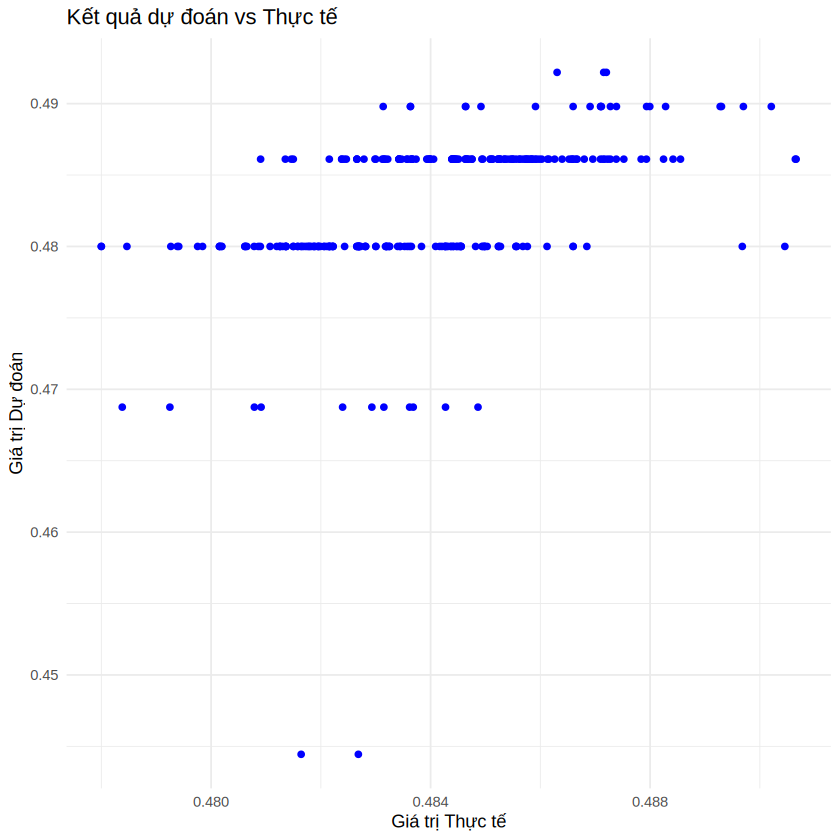
\includegraphics[width=0.75\columnwidth]{wine_figures/red_pred.png}
    \caption{Kết quả dự đoán trên bộ dữ liệu chất lượng rượu đỏ.}
    \label{fig:red_pred}
\end{figure}


\subsection{Phân tích chất lượng rượu (bao gồm nhiều tố màu sắc)}


\subsubsection{Các thông tin thống kê mô tả về tập dữ liệu}


\subsubsection{Phân tích đơn biến}

% Chất lượng rượu
\textbf{Chất lượng rượu}
\begin{figure}[H]
    \centering
    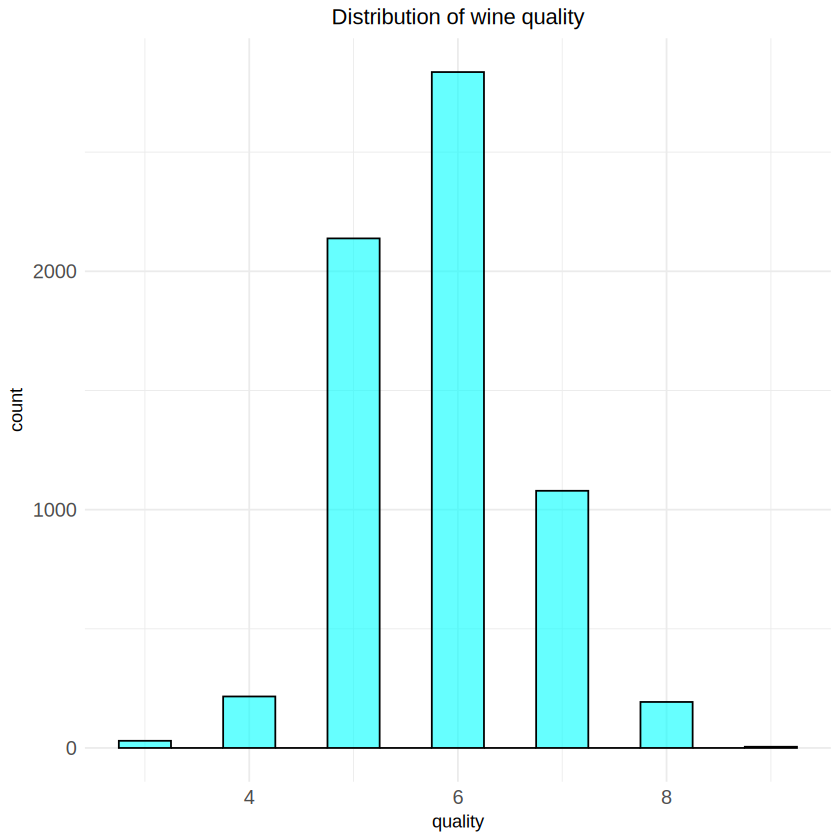
\includegraphics[width=0.75\columnwidth]{wine_colors/wine_quality.png}
    \caption{Chất lượng rượu.}
    \label{fig:wine_quality}
\end{figure}
Nhận xét:
\begin{itemize}
    \item Chất lượng rượu có phân phối đối xứng 
    \item Hầu hết chất lượng rượu đỏ nằm ở mức 5, 6
    \item Không có rượu đỏ nào đạt điểm tuyệt đối
    \item Chất lượng rượu đỏ tệ nhất có điểm số là 3
\end{itemize}

% Khảo sát tính chua (acidity) trong rượu
\textbf{Khảo sát tính chua (acidity) trong rượu}
\begin{figure}[H]
    \centering
    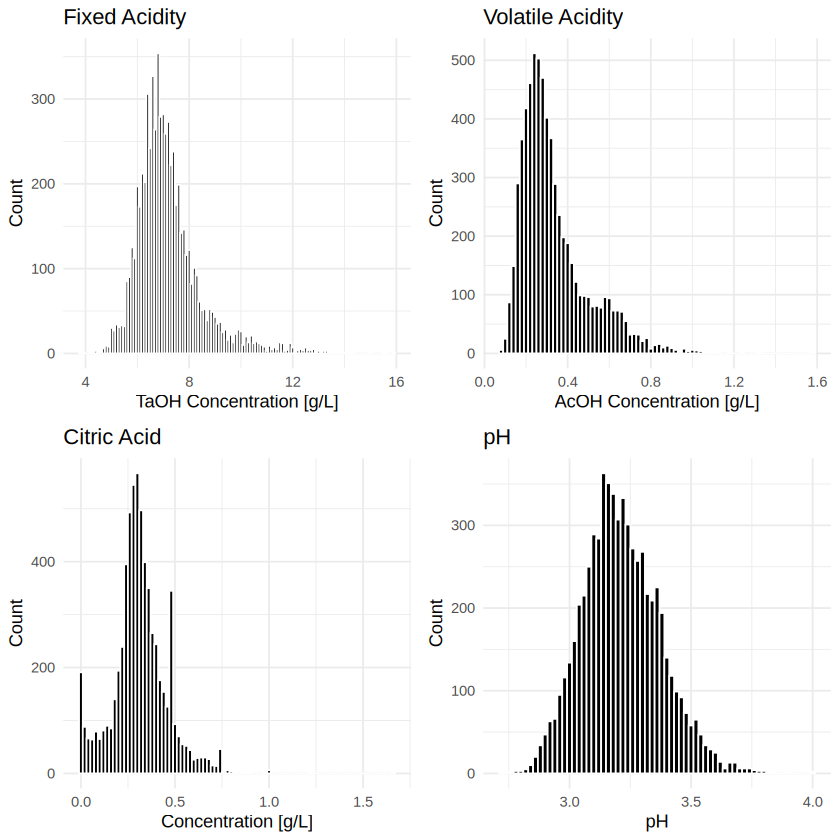
\includegraphics[width=0.75\columnwidth]{wine_colors/wine_acidity.png}
    \caption{Histogram tính chua (acidity) trong rượu.}
    \label{fig:wine_acidity}
\end{figure}
Nhận xét:
\begin{itemize}
    \item Độ axit cố định (fixed acidity) và dễ bay hơi (volatile acidity) cho thấy sự phân bố lệch dương (lệch phải). Axit xitric tạo thành sự phân bố đỉnh cạnh vì một nhóm rượu vang dường như có nồng độ axit xitric gần bằng 0. Biểu đồ pH có vẻ đối xứng hơn. Chỉ có một vài giá trị ngoại lệ có mặt xuất hiện ở các đặc trưng này.
\end{itemize}

\begin{figure}[H]
    \centering
    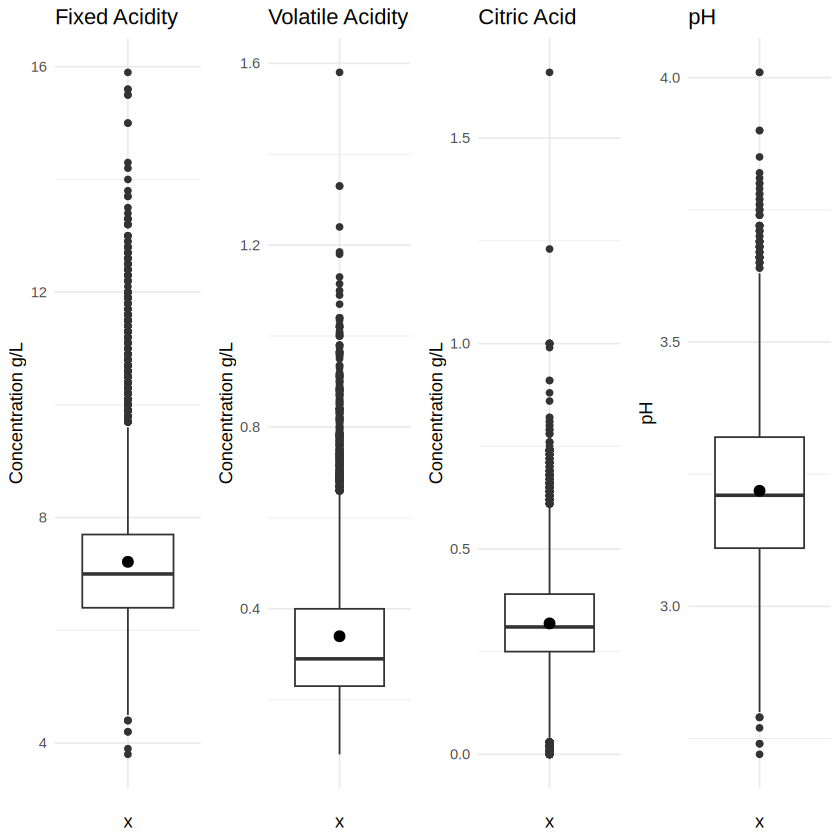
\includegraphics[width=0.75\columnwidth]{wine_colors/wine_acidity_boxplot.png}
    \caption{Boxplot tính chua (acidity) trong rượu.}
    \label{fig:wine_acidity_boxplot}
\end{figure}
Nhận xét:
\begin{itemize}
    \item Nhìn vào các thông số độ axit trong biểu đồ hộp cho thấy một hình ảnh tương tự. Người ta có thể thấy đuôi dương dài của nồng độ axit cố định và dễ bay hơi và phân phối hẹp hơn đối với axit citric và độ pH. Quan sát này cũng được xác nhận bởi các giá trị trung bình được hiển thị bằng dấu chấm đen trong biểu đồ. Chúng gần với các giá trị trung bình tương ứng đối với axit citric và độ pH hơn là đối với độ axit cố định và dễ bay hơi.
\end{itemize}

% Khảo sát hàm lượng lưu huỳnh trong rượu
\textbf{Khảo sát hàm lượng lưu huỳnh trong rượu}
\begin{figure}[H]
    \centering
    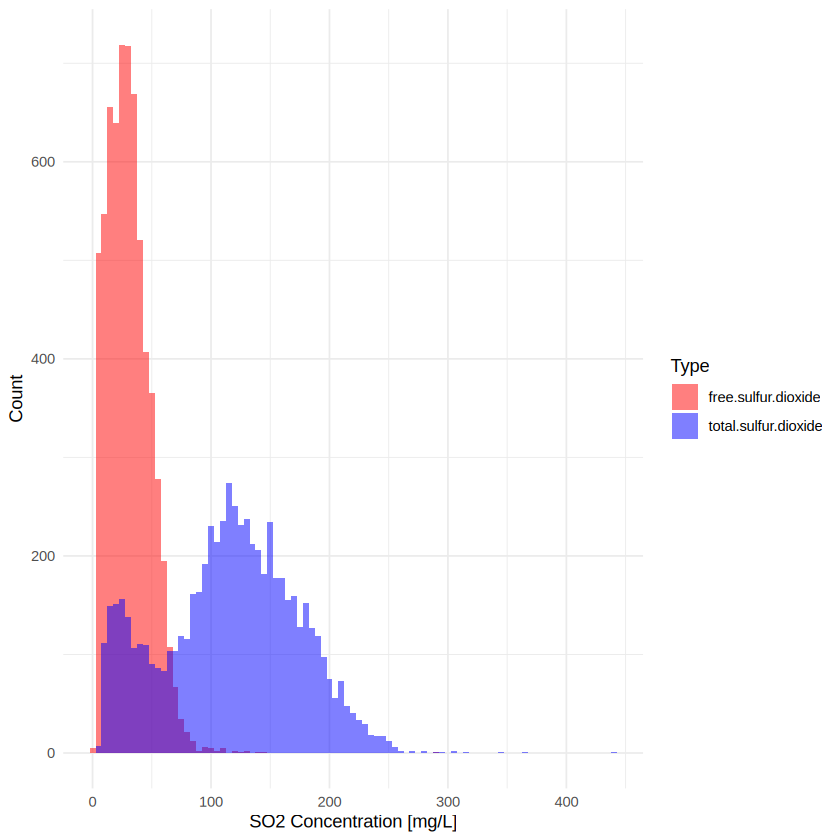
\includegraphics[width=0.75\columnwidth]{wine_colors/wine_sulfur.png}
    \caption{Phân phối SO2 tự do và tổng lượng SO2 trong rượu.}
    \label{fig:wine_sulfur_dis}
\end{figure}
Nhận xét:
\begin{itemize}
    \item Nồng độ lưu huỳnh dioxit tự do tập trung hẹp quanh mức 30 mg/L. Nồng độ lưu huỳnh dioxit tổng thể cho thấy dấu hiệu lưỡng cực với các đỉnh quanh mức 20 và 120 mg/L.
\end{itemize}

\begin{figure}[H]
    \centering
    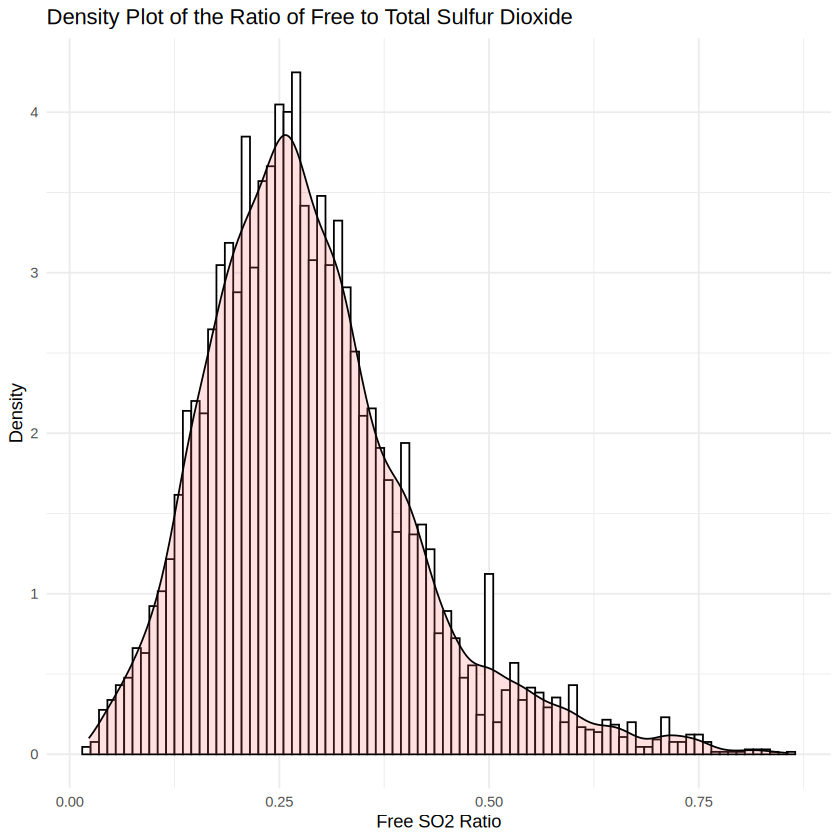
\includegraphics[width=0.75\columnwidth]{wine_colors/wine_ratio_sulfur.png}
    \caption{Phân phối tỷ lệ SO2 tự do và tổng lượng SO2.}
    \label{fig:wine_ratio_sulfur}
\end{figure}
Nhận xét:
\begin{itemize}
    \item Khi vẽ biểu đồ tỷ lệ giữa lưu huỳnh dioxit tự do và lưu huỳnh dioxit tổng trong rượu vang, người ta có thể thấy rằng khoảng 30\% lưu huỳnh dioxit tổng xuất hiện ở dạng tự do. Sự phân bố bị lệch dương với một số loại rượu vang có tỷ lệ cao hơn đáng kể. Điểm đáng chú ý nữa là đỉnh xuất hiện chính xác ở mức 0,5.
\end{itemize}

\begin{figure}[H]
    \centering
    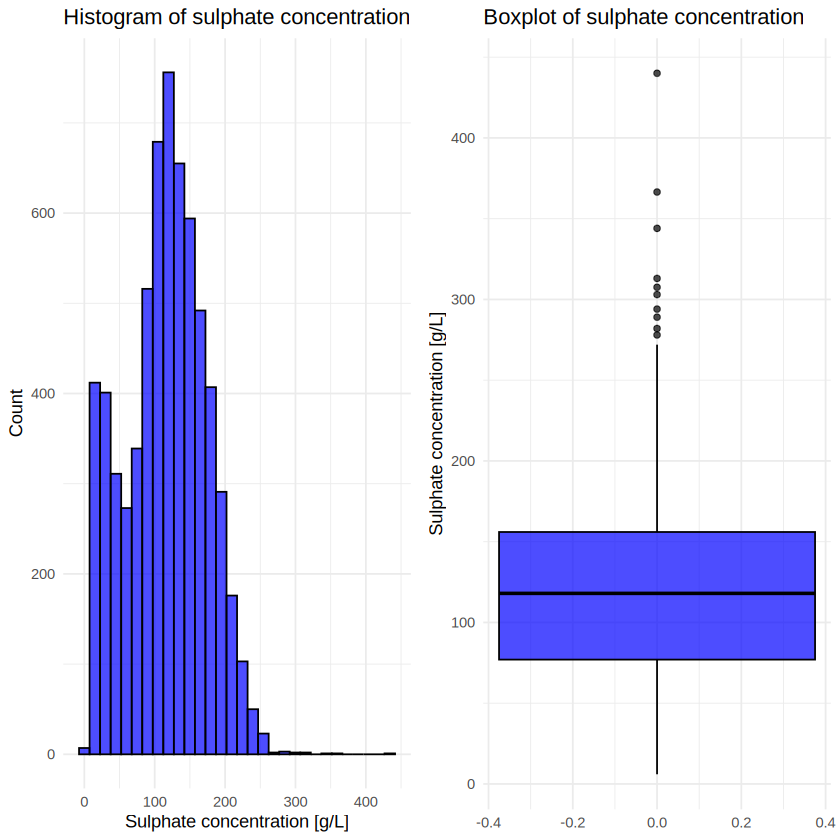
\includegraphics[width=0.75\columnwidth]{wine_colors/wine_sulphate.png}
    \caption{Phân phối Lượng muối sunphat trong rượu.}
    \label{fig:wine_sulphate}
\end{figure}
Nhận xét:
\begin{itemize}
    \item Hầu hết các loại rượu vang có nồng độ sulfat khoảng 0,5 g/L. Có thể thấy hai nhóm ngoại lệ nhỏ khoảng 1,6 và 1,9 g/L trong biểu đồ hộp.
\end{itemize}

% Khảo sát lượng đường còn lại sau khi lên men trong rượu
\textbf{Khảo sát lượng đường còn lại sau khi lên men trong rượu}
\begin{figure}[H]
    \centering
    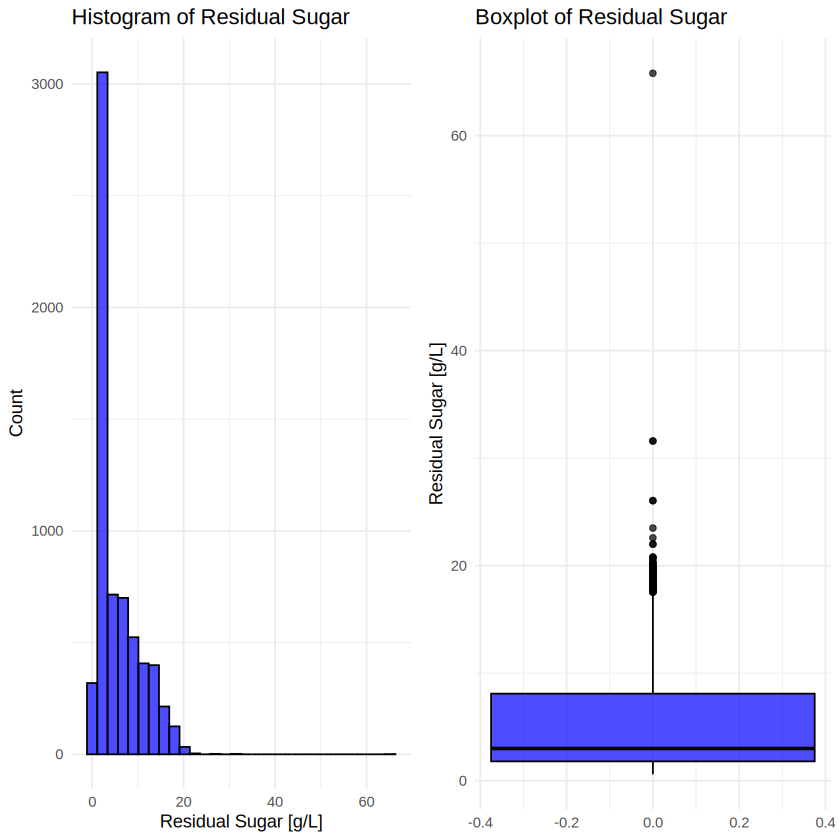
\includegraphics[width=0.75\columnwidth]{wine_colors/wine_sugar.png}
    \caption{Phân phối lượng đường còn lại sau khi lên men trong rượu.}
    \label{fig:wine_sugar}
\end{figure}
Nhận xét:
\begin{itemize}
    \item  Nhìn chung, các loại rượu vang trong tập dữ liệu có vẻ có nồng độ đường dư thấp. Độ lệch dương di chuyển giá trị trung bình (5,4) lên trên giá trị trung vị (3,0). Có thể tìm thấy giá trị ngoại lệ cực độ xung quanh 65 g/L đường dư
\end{itemize}

% Khảo sát phần trăm cồn trong rượu
\textbf{Khảo sát phần trăm cồn trong rượu}
\begin{figure}[H]
    \centering
    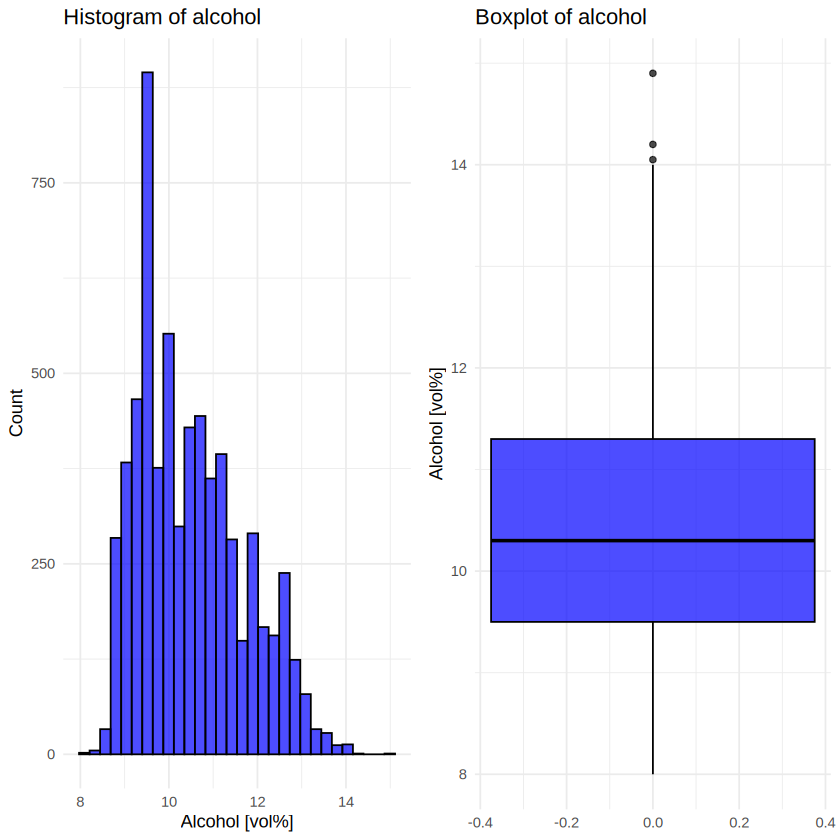
\includegraphics[width=0.75\columnwidth]{wine_colors/wine_alcohol.png}
    \caption{Phân phối phần trăm cồn trong rượu.}
    \label{fig:wine_alcohol}
\end{figure}
Nhận xét:
\begin{itemize}
    \item Hàm lượng cồn của rượu vang trong tập dữ liệu dao động từ 8 đến 15 vol\%. Giá trị trung bình nằm trong khoảng 10 vol. Phân phối khá rộng và cho thấy độ lệch dương (lệch phải).
\end{itemize}

% Khảo sát mật độ trong rượu
\textbf{Khảo sát mật độ trong rượu}
\begin{figure}[H]
    \centering
    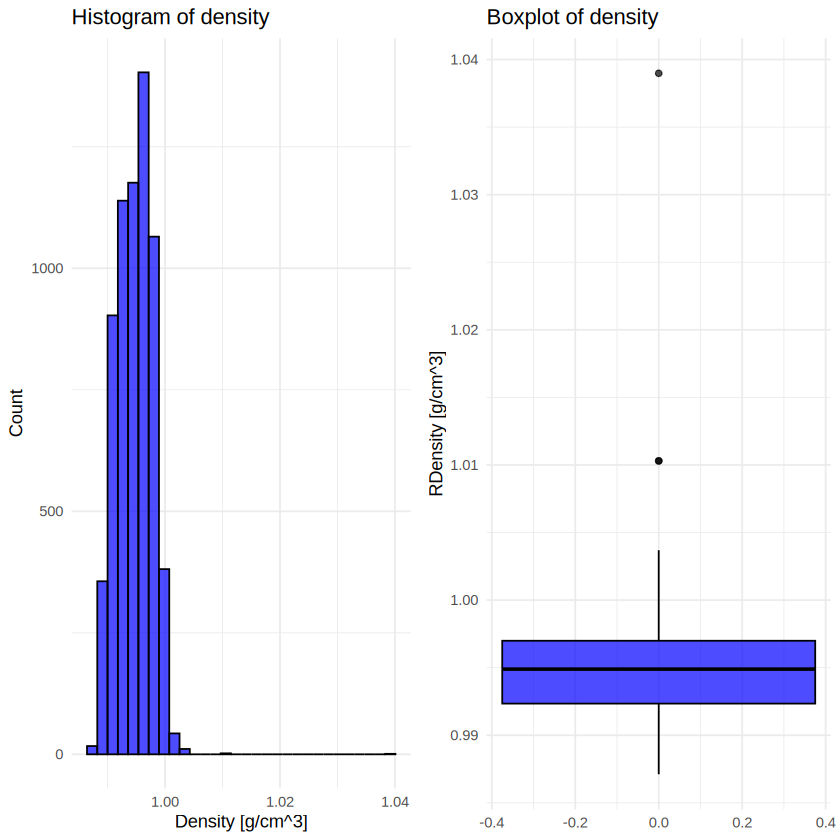
\includegraphics[width=0.75\columnwidth]{wine_colors/wine_density.png}
    \caption{Phân phối mật độ rượu.}
    \label{fig:wine_density}
\end{figure}
Nhận xét:
\begin{itemize}
    \item Tham số mật độ cho thấy sự phân bố rất hẹp với sự thay đổi thấp. Người ta có thể thấy một vài giá trị ngoại lệ trong khoảng 1,01 và 1,04 g/cm3 nhưng hầu hết các loại rượu vang có mật độ trong khoảng 0,99 và 1,00 g/cm3.
\end{itemize}

% Khảo sát lượng muối trong rượu
\textbf{Khảo sát lượng muối trong rượu}
\begin{figure}[H]
    \centering
    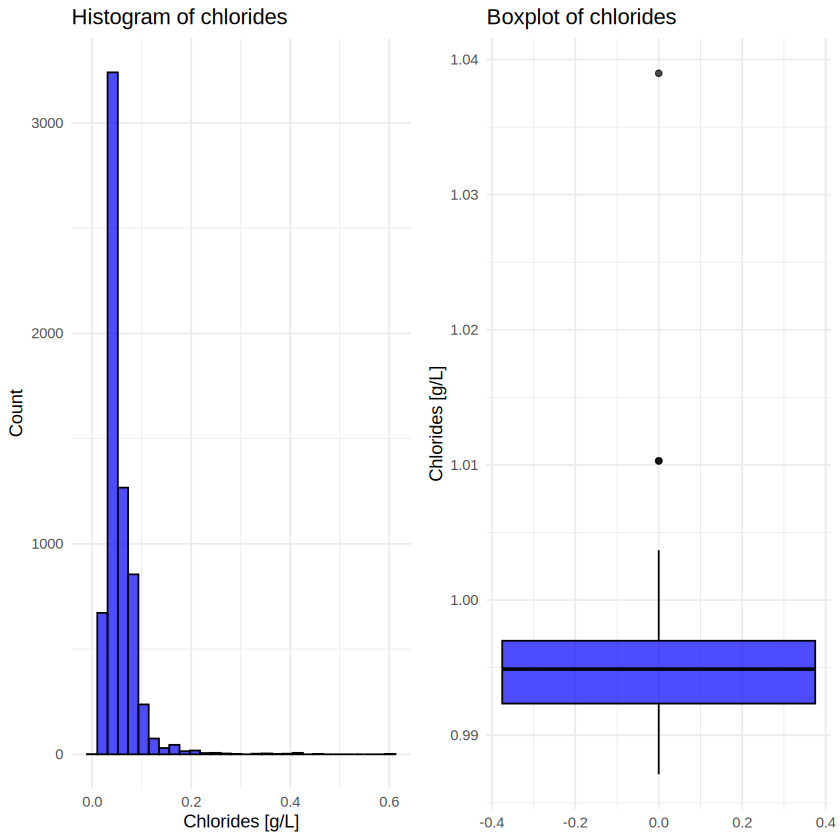
\includegraphics[width=0.75\columnwidth]{wine_colors/wine_chlorides.png}
    \caption{Phân phối lượng muối rượu.}
    \label{fig:wine_chlorides}
\end{figure}
Nhận xét:
\begin{itemize}
    \item Biểu đồ histogram cho thấy nồng độ clo trong tập dữ liệu có hai đỉnh chính riêng biệt. Nồng độ clo thường gặp nhất có thể được tìm thấy ở khoảng 0,04 g/L. Đỉnh thứ hai xuất hiện ở khoảng 0,08 g/L. Phân phối có đuôi rất dài theo hướng tích cực với các giá trị ngoại lệ lên đến 0,6 g/L.
\end{itemize}

Tiểu kết phần phân tích đơn biến. Một số nhận xét chính:
\begin{itemize}
    \item Hầu hết các loại rượu vang đều có xếp hạng chất lượng là 6. Không có loại rượu nào đạt điểm tối đa là 10.
    \item Độ axit được đo bằng các thành phần cố định và dễ bay hơi. Hầu hết các loại rượu vang đều có độ pH là 3,2.
    \item Nồng độ lưu huỳnh dioxit thay đổi rất nhiều trong các loại rượu vang được nghiên cứu.
    \item Các loại rượu vang có hàm lượng cồn dao động từ 8 đến 15 vol\%. Nồng độ clorua cho thấy sự phân bố bimodal với các đỉnh ở 0,04 và 0,08 g/L.
\end{itemize}

\subsubsection{Phân tích ma trận tương quan}

\begin{figure}[H]
    \centering
    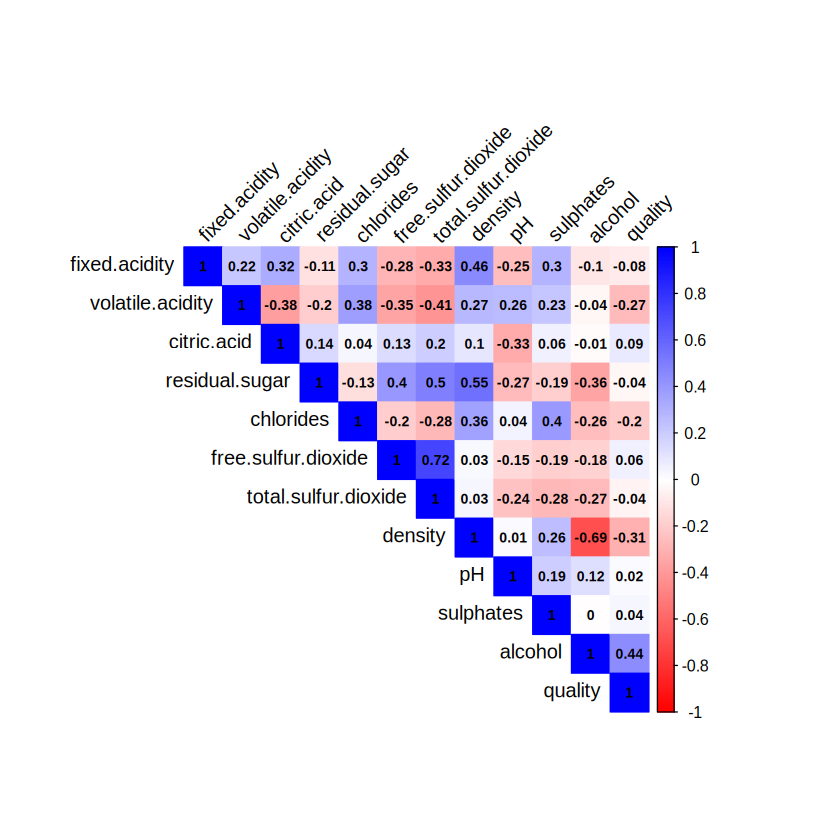
\includegraphics[width=0.75\columnwidth]{wine_colors/wine_corr.png}
    \caption{Ma trận tương quan giữa các biến trong tập dữ liệu về rượu.}
    \label{fig:wine_corr}
\end{figure}
Nhận xét:
\begin{itemize}
    \item Chọn ngưỡng là 0.3, ta thấy:
    \begin{itemize}
        \item Nồng độ cồn (alcohol) có ảnh hưởng (thuận) đến chất lượng rượu (chỉ số tương quan 0.436)
        \item Các biến `residual.sugar` và `density` có tương quan thuận cao 0.83
        \item Mật độ trong rượu (`density`) có ảnh hưởng (nghịch) đến chất lượng của rượu (chỉ số tương quan -0.307)
        \item Các biến `alcohol` và `density` có tương quan nghịch cao -0.78
    \end{itemize}
\end{itemize}

\subsubsection{Phân tích ảnh hưởng của các biến đối với chất lượng rượu}

\textbf{Khảo sát mối quan hệ giữa Density và Quality}
\begin{figure}[H]
    \centering
    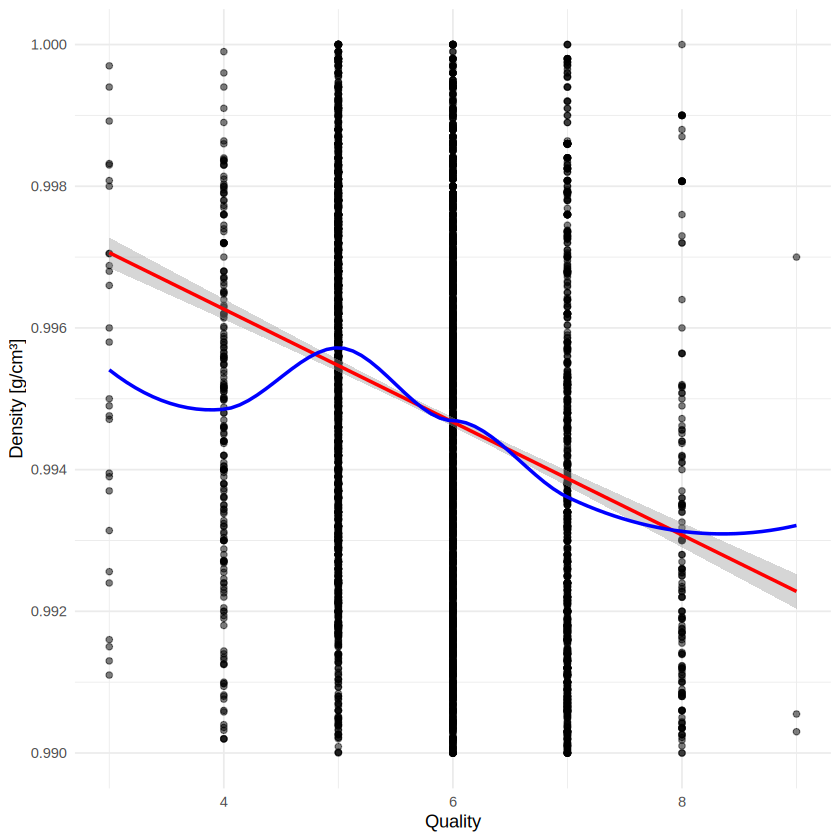
\includegraphics[width=0.75\columnwidth]{wine_colors/wine_density_quality.png}
    \caption{Mối quan hệ giữa .Density và Quality}
    \label{fig:wine_density_quality}
\end{figure}
Nhận xét:
\begin{itemize}
    \item Biểu đồ trên cho thấy mật độ rượu được nhóm theo xếp hạng chất lượng của chúng. 
    \item Các giá trị ngoại lệ có thể bị bỏ qua do scale trục y. 
    \item Đường màu xanh lam kết nối các giá trị trung bình của các nhóm chất lượng khác nhau trong khi một đường xu hướng tuyến tính được thêm vào màu đỏ. Chúng ta có thể quan sát thấy xu hướng tiêu cực giữa mật độ và chất lượng nhưng vì chúng ta có các biến thể mật độ lớn trong các nhóm chất lượng khác nhau nên tôi không mong đợi mật độ là một biến dự báo tốt cho chất lượng rượu.
\end{itemize}

\begin{figure}[H]
    \centering
    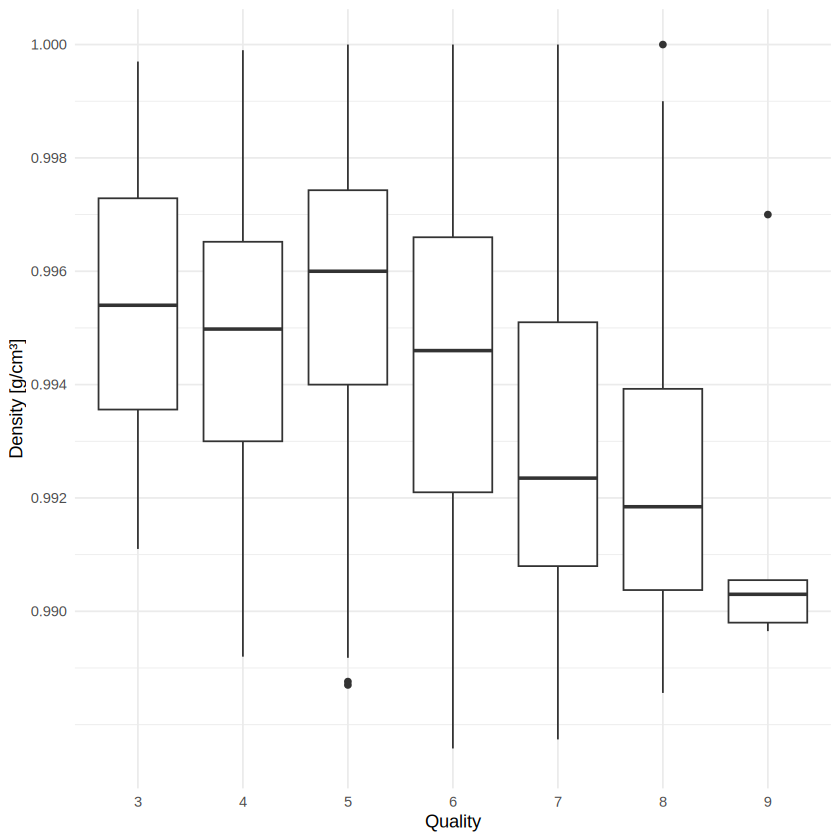
\includegraphics[width=0.75\columnwidth]{wine_colors/wine_density_quality_boxplot.png}
    \caption{Biểu đồ boxplot về mối quan hệ giữa Density và Quality}
    \label{fig:wine_density_quality_boxplot}
\end{figure}
Nhận xét:
\begin{itemize}
    \item Chúng ta có được một số nhận định tương tự khi hình dung mối quan hệ giữa chất lượng và mật độ bằng biểu đồ hộp. 
    \item Rượu có mật độ thấp hơn có xu hướng có chất lượng tốt hơn nhưng mật độ thay đổi trong các cửa sổ tương tự trong tất cả các nhóm chất lượng.
\end{itemize}

\textbf{Khảo sát mối quan hệ giữa Alcohol và Quality}
\begin{figure}[H]
    \centering
    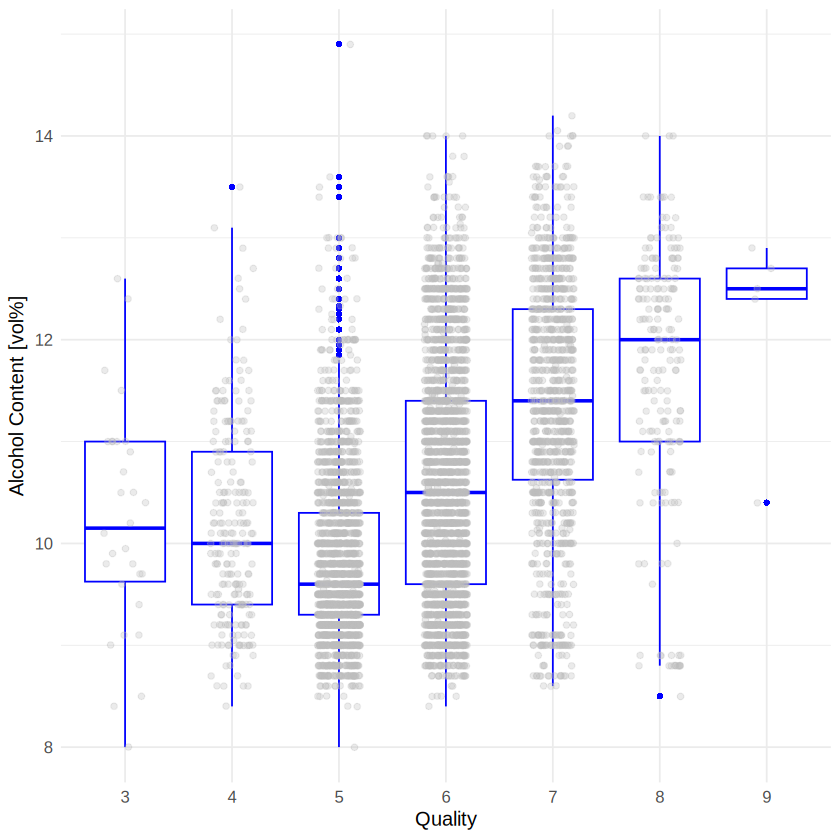
\includegraphics[width=0.75\columnwidth]{wine_colors/wine_alcohol_quality.png}
    \caption{Mối quan hệ giữa Alcoholy và Quality}
    \label{fig:wine_alcohol_quality}
\end{figure}
Nhận xét:
\begin{itemize}
    \item Biểu đồ hộp cho thấy rượu vang có chất lượng cao hơn có vẻ có nồng độ cồn cao hơn. Nhưng mối quan hệ này có vẻ không đáng kể vì các hộp rất rộng và chồng chéo lên nhau đối với các loại khác nhau.
\end{itemize}

\textbf{Khảo sát mối quan hệ giữa Chlorides và Quality}
\begin{figure}[H]
    \centering
    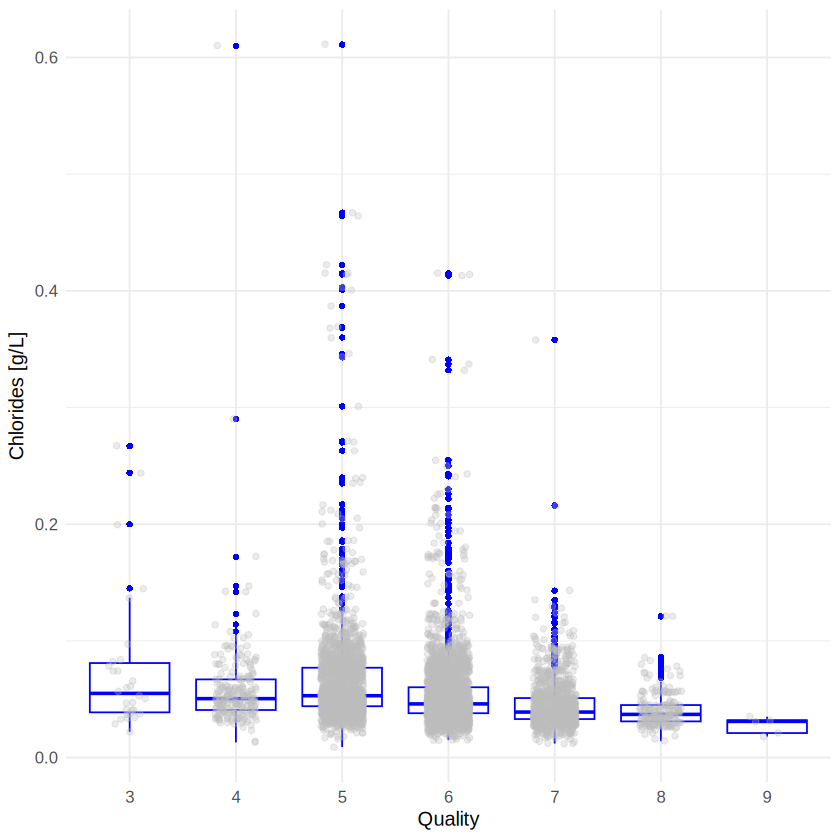
\includegraphics[width=0.75\columnwidth]{wine_colors/wine_chlorides_quality.png}
    \caption{Mối quan hệ giữa Chlorides và Quality}
    \label{fig:wine_chlorides_quality}
\end{figure}
Nhận xét:
\begin{itemize}
    \item Rượu vang có nồng độ clorua thấp hơn có xu hướng có chất lượng tốt hơn nhưng hiệu ứng có vẻ rất yếu. Các khối hộp rộng và ta có thể thấy rất nhiều ngoại lệ đối với rượu vang chất lượng trung bình.
\end{itemize}

\textbf{Khảo sát mối quan hệ giữa Volatile Acidity và Quality}
\begin{figure}[H]
    \centering
    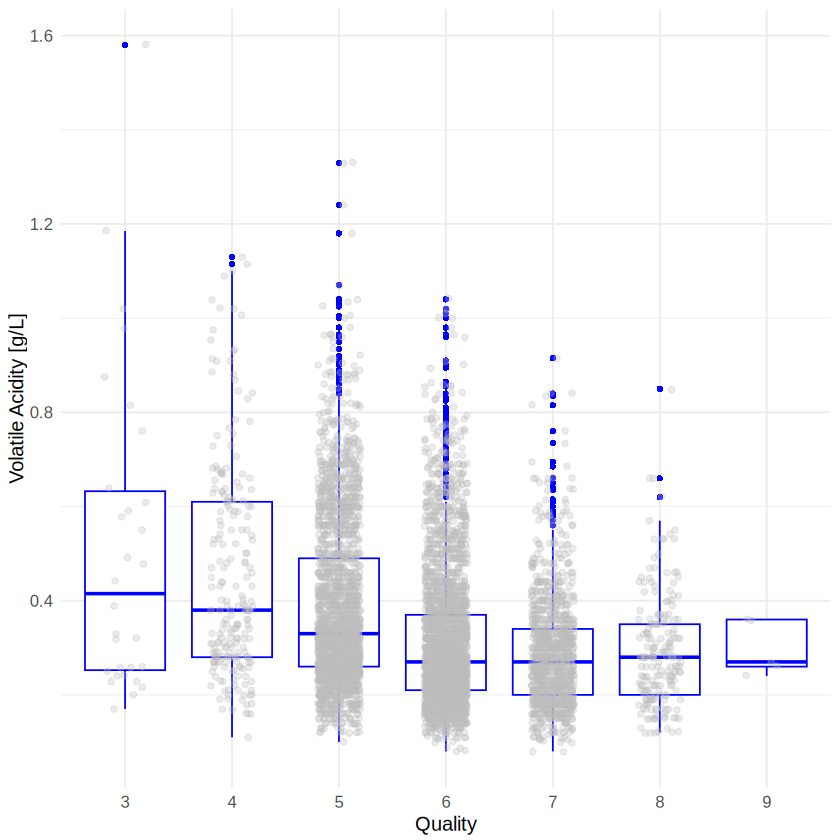
\includegraphics[width=0.75\columnwidth]{wine_colors/wine_volatile_acidity_quality.png}
    \caption{Mối quan hệ giữa Volatile Acidity và Quality}
    \label{fig:wine_volatile_acidity_quality}
\end{figure}
Nhận xét:
\begin{itemize}
    \item Một lần nữa chúng ta chỉ có thể thấy mối tương quan âm rất yếu trong việc hình dung nồng độ axit axetic so với chất lượng rượu.
\end{itemize}

\textbf{Khảo sát mối quan hệ giữa tổng lượng SO2 và lượng đường còn lại sau khi lên men}
\begin{figure}[H]
    \centering
    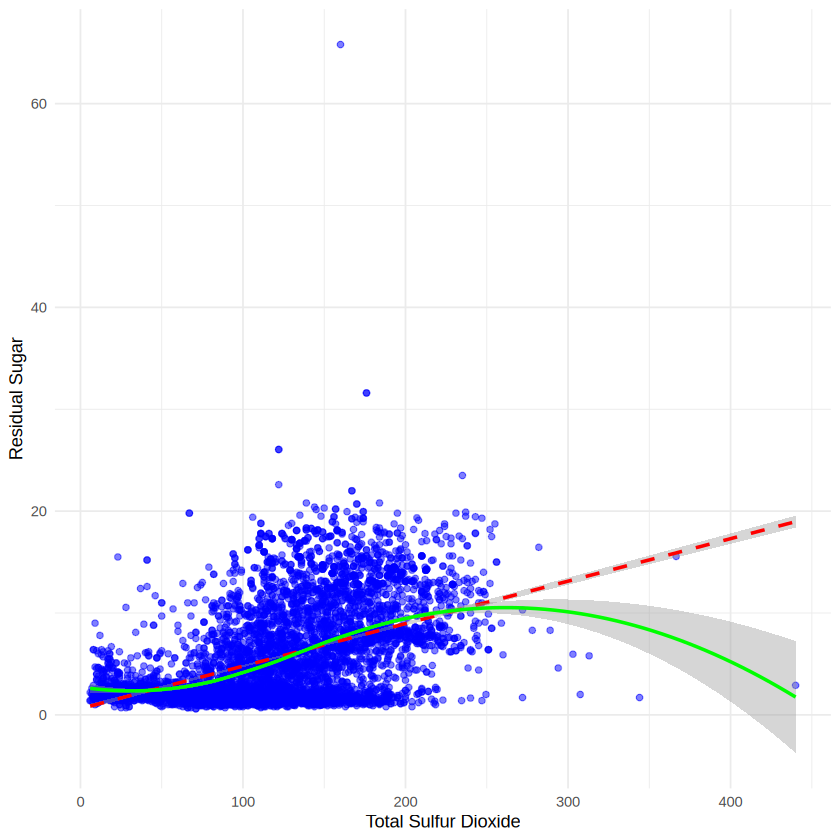
\includegraphics[width=0.75\columnwidth]{wine_colors/wine_sulfur_sugar.png}
    \caption{Mối quan hệ giữa tổng lượng SO2 và lượng đường còn lại sau khi lên men}
    \label{fig:wine_sulfur_sugar}
\end{figure}
Nhận xét:
\begin{itemize}
    \item Đối với phần lớn rượu vang, nồng độ lưu huỳnh dioxit tổng thể dường như không bị ảnh hưởng bởi lượng đường còn lại. Chúng ta có thể thấy rằng rượu vang trải dài toàn bộ phạm vi nồng độ lưu huỳnh dioxit đối với mức đường còn lại thấp. Nhưng có vẻ như rượu vang có lượng đường còn lại cao cũng thường có nồng độ lưu huỳnh dioxit tổng thể cao.
\end{itemize}

\textbf{Khảo sát tác động của nồng độ cồn, đường dư và lượng đường đến mật độ rượu}
\begin{figure}[H]
    \centering
    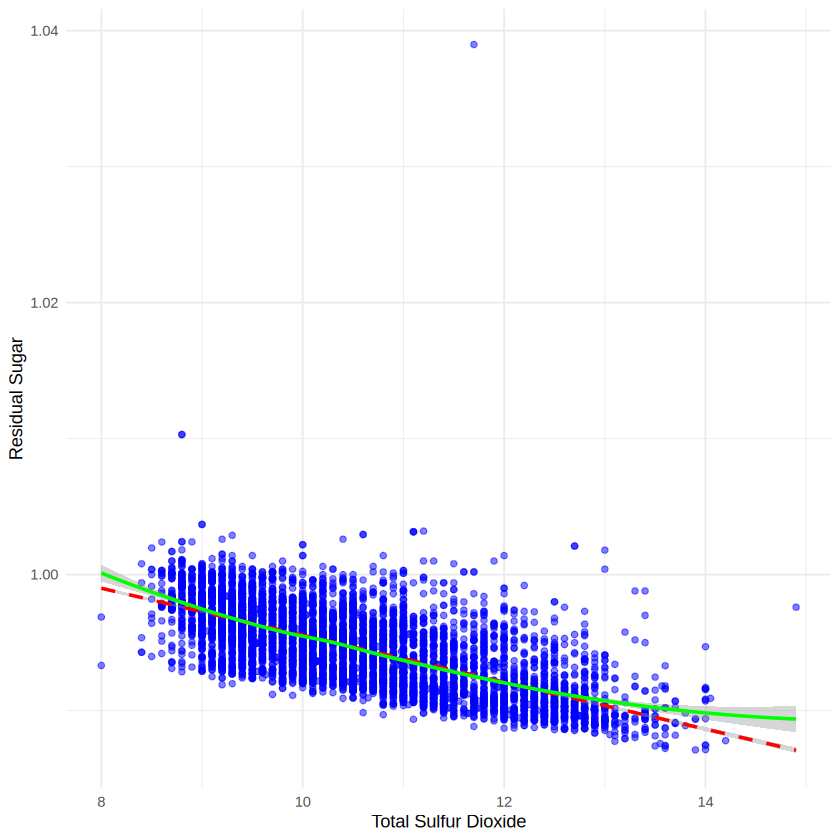
\includegraphics[width=0.75\columnwidth]{wine_colors/wine_alcohol_density.png}
    \caption{Mối quan hệ giữa nồng độ cồn và lượng đường đến mật độ rượu}
    \label{fig:wine_alcohol_density}
\end{figure}

\begin{figure}[H]
    \centering
    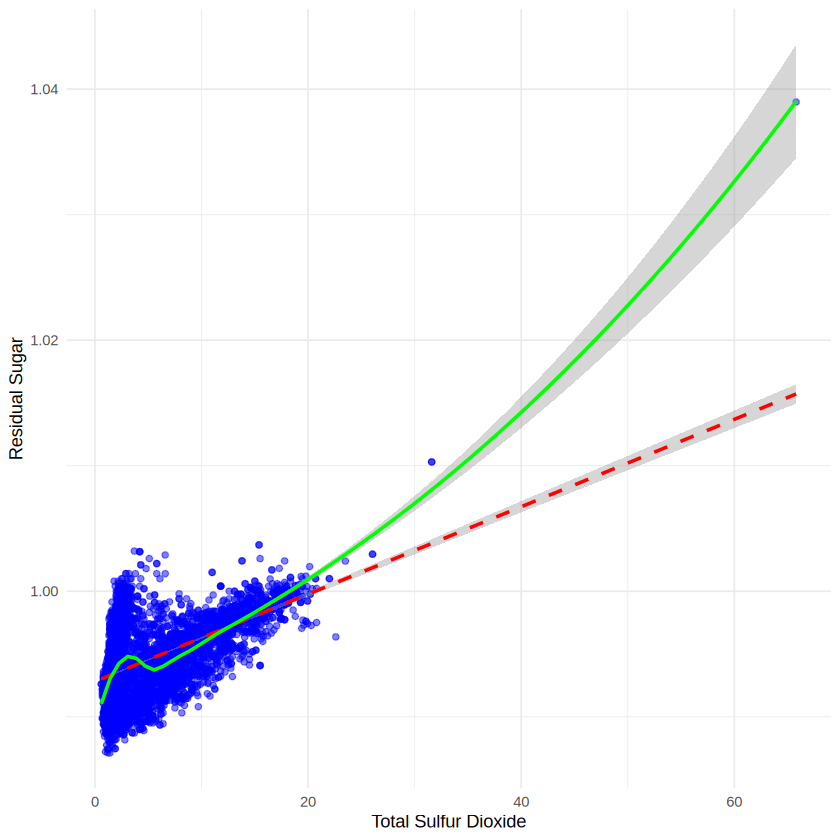
\includegraphics[width=0.75\columnwidth]{wine_colors/wine_sugar_density.png}
    \caption{Mối quan hệ giữa đường dư và lượng đường đến mật độ rượu}
    \label{fig:wine_sugar_density}
\end{figure}

Nhận xét:
\begin{itemize}
    \item Nồng độ cồn cũng như nồng độ đường còn lại cho thấy ảnh hưởng dự kiến đến mật độ rượu.
    \item Nồng độ cồn cao hơn làm giảm mật độ rượu trong khi lượng đường còn lại nhiều hơn làm tăng mật độ.
    \item  Đường có mật độ cao hơn nước và do đó làm tăng mật độ của hỗn hợp trong khi rượu thì ngược lại.
\end{itemize}

\subsubsection{Phân tích dựa trên màu sắc của rượu}

\textbf{Phân tích mối quan hệ giữa màu sắc và mật độ rượu}
\begin{figure}[H]
    \centering
    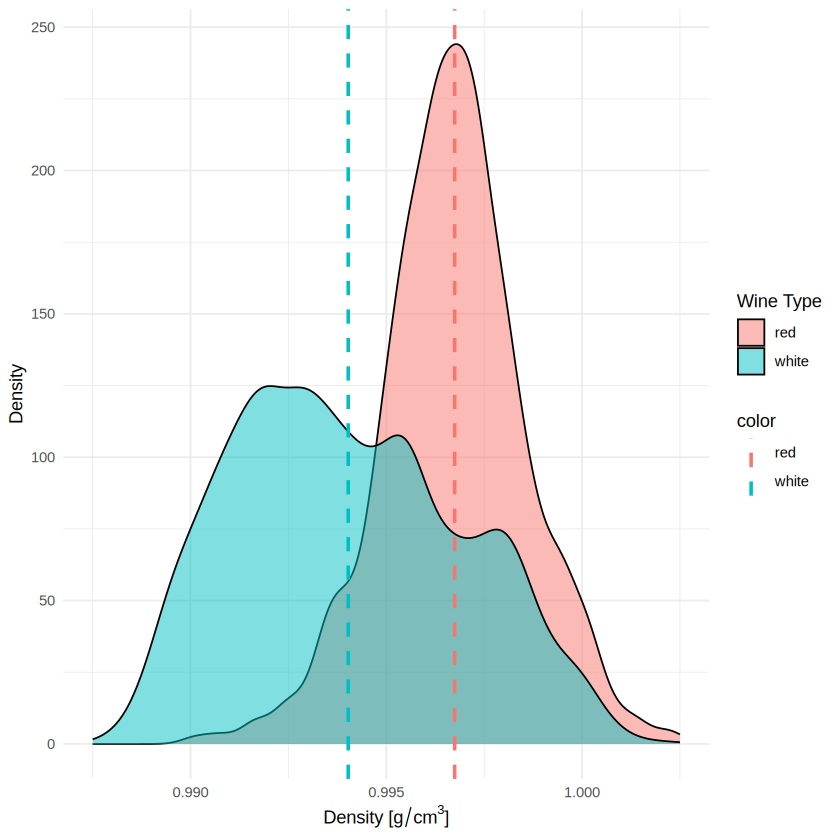
\includegraphics[width=0.75\columnwidth]{wine_colors/wine_color_density.png}
    \caption{Mối quan hệ giữa màu sắc và mật độ rượu}
    \label{fig:wine_color_density}
\end{figure}
Nhận xét:
\begin{itemize}
    \item Trong biểu đồ phân bố mật độ ở trên, ta có thể thấy rằng rượu vang trắng và rượu vang đỏ có mật độ khác nhau. Rượu vang đỏ có sự phân bố khá hẹp với giá trị trung bình khoảng 0,997 g/cm3. Ngược lại, rượu vang trắng có sự thay đổi mật độ rộng hơn nhiều nhưng trung bình của chúng nằm dưới giá trị trung bình của rượu vang đỏ khoảng 0,993 g/cm3.
\end{itemize}

\textbf{Phân tích mối quan hệ giữa màu sắc và lượng đường còn lại sau khi lên men}
\begin{figure}[H]
    \centering
    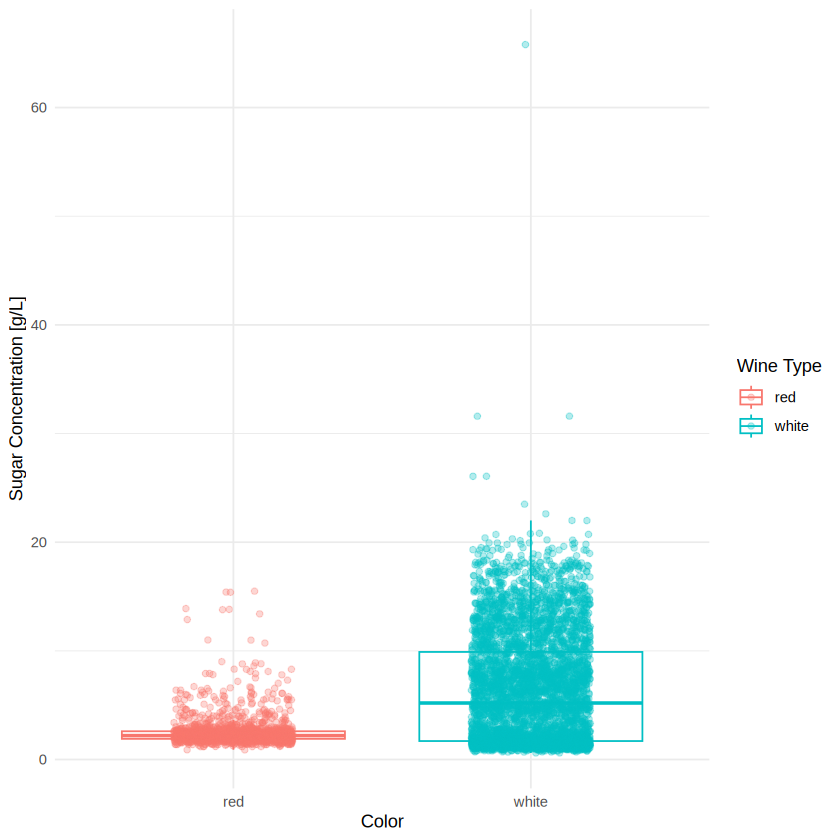
\includegraphics[width=0.75\columnwidth]{wine_colors/wine_color_sugar.png}
    \caption{Mối quan hệ giữa màu sắc và lượng đường còn lại sau khi lên men}
    \label{fig:wine_color_sugar}
\end{figure}
Nhận xét:
\begin{itemize}
    \item Nồng độ đường còn lại thấp hơn ở rượu vang đỏ so với rượu vang trắng và sự phân bố của chúng hẹp hơn.
\end{itemize}

\textbf{Phân tích mối quan hệ giữa màu sắc và tổng lượng lưu huỳnh trong rượu}
\begin{figure}[H]
    \centering
    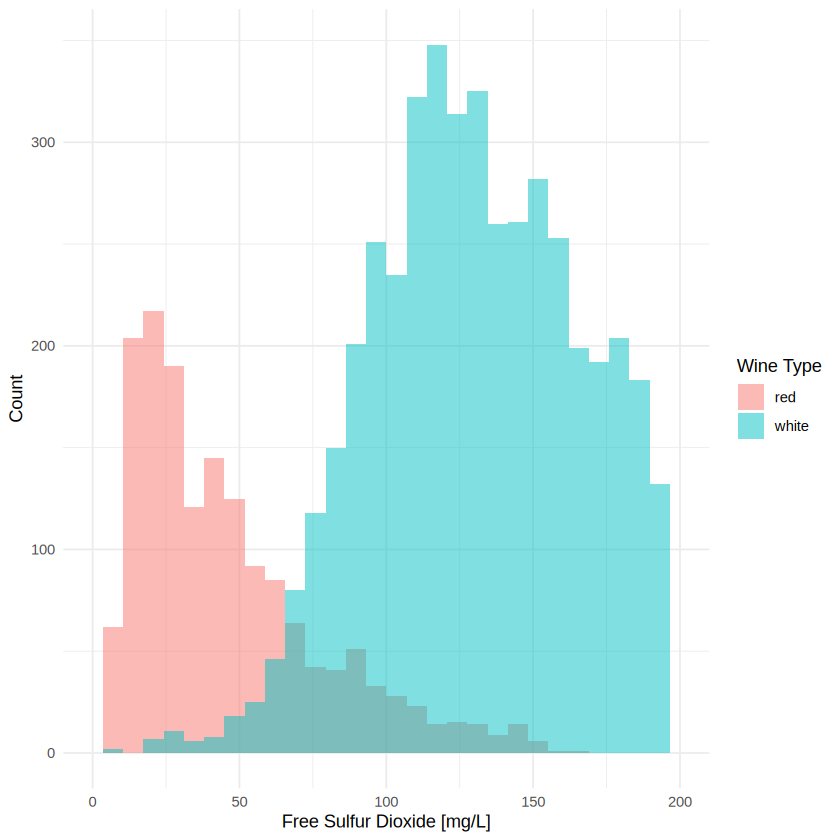
\includegraphics[width=0.75\columnwidth]{wine_colors/wine_color_sulfur.png}
    \caption{Mối quan hệ giữa màu sắc và tổng lượng lưu huỳnh trong rượu}
    \label{fig:wine_color_sulfur}
\end{figure}
Nhận xét:
\begin{itemize}
    \item Biểu đồ ở trên cho thấy mối quan hệ giữa màu rượu vang và nồng độ lưu huỳnh đioxit tổng thể. Hầu hết rượu vang đỏ có nồng độ lưu huỳnh đioxit tổng thể thấp trong khi rượu vang trắng cho thấy sự phân bố đối xứng xung quanh giá trị trung bình cao hơn là 130 g/L.
\end{itemize}

\textbf{Phân tích mối quan hệ giữa màu sắc và lượng lưu huỳnh tự do trong rượu}
\begin{figure}[H]
    \centering
    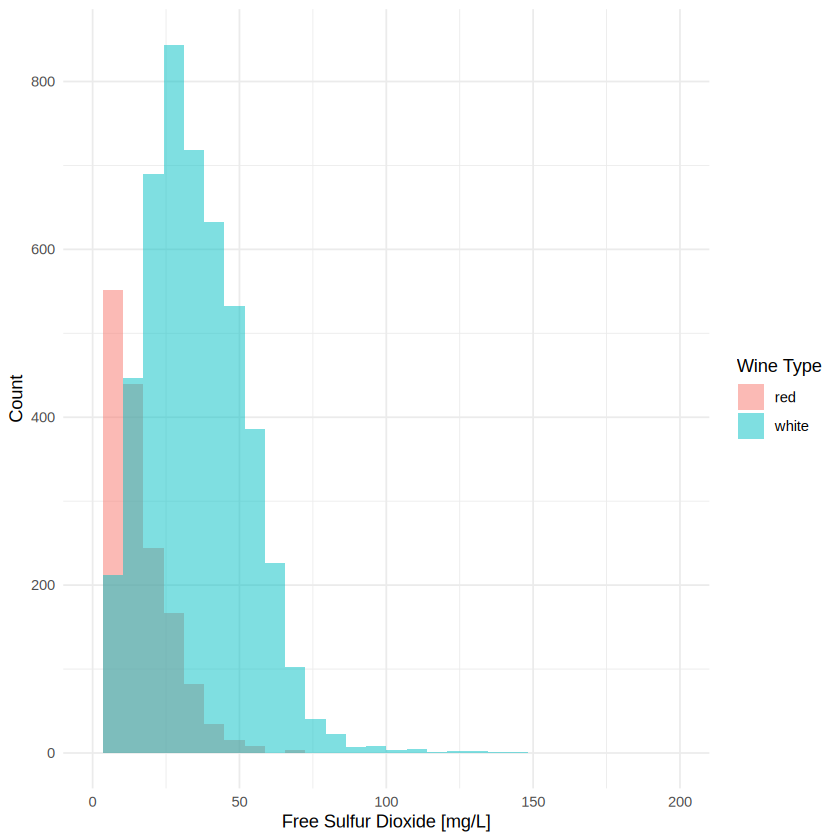
\includegraphics[width=0.75\columnwidth]{wine_colors/wine_color_freesulfur.png}
    \caption{Mối quan hệ giữa màu sắc và lượng lưu huỳnh tự do trong rượu}
    \label{fig:wine_color_freesulfur}
\end{figure}
Nhận xét:
\begin{itemize}
    \item Khi xem xét sự khác biệt giữa lưu huỳnh đioxit tổng và tự do, chúng ta có thể khẳng định rõ ràng rằng lưu huỳnh đioxit cố định là nguyên nhân tạo nên sự khác biệt về màu sắc của rượu vang.
\end{itemize}

\textbf{Phân tích mối quan hệ giữa màu sắc và tính chua của rượu}
\begin{figure}[H]
    \centering
    \includegraphics[width=0.75\columnwidth]{wine_colors/wine_color_volatile_acidity.png}
    \caption{Mối quan hệ giữa màu sắc và tính chua của rượu}
    \label{fig:wine_color_volatile_acidity}
\end{figure}
Nhận xét:
\begin{itemize}
    \item Sự phân bố của độ axit dễ bay hơi cho thấy đỉnh chính của nó ở nồng độ thấp hơn đối với rượu vang trắng so với rượu vang đỏ. Trong khi đường cong đối với rượu vang trắng hẹp với độ lệch dương, đường cong mật độ rượu vang đỏ rộng và cho thấy dấu hiệu của phân phối hai đỉnh.
\end{itemize}

\subsubsection{Phân tích tương quan giữa các biến dựa trên màu sắc}

\textbf{Khảo sát tương quan giữa mật độ và chất lượng rượu dựa trên màu sắc}
\begin{figure}[H]
    \centering
    \includegraphics[width=0.75\columnwidth]{wine_colors/wine_density_quality_color.png}
    \caption{Mối quan hệ giữa mật độ và chất lượng rượu dựa trên màu sắc}
    \label{fig:wine_density_quality_color}
\end{figure}
Nhận xét:
\begin{itemize}
    \item Đối với cả hai nhóm rượu, chất lượng có tương quan nghịch với mật độ. Nhưng tác dụng có vẻ mạnh hơn một chút đối với rượu vang trắng.
\end{itemize}

\textbf{Khảo sát tương quan giữa nồng độ cồn và chất lượng rượu dựa trên màu sắc}
\begin{figure}[H]
    \centering
    \includegraphics[width=0.75\columnwidth]{wine_colors/wine_alcohol_quality_color.png}
    \caption{Mối quan hệ giữa nồng độ cồn và chất lượng rượu dựa trên màu sắc}
    \label{fig:wine_alcohol_quality_color}
\end{figure}
Nhận xét:
\begin{itemize}
    \item Ngoài ra đối với nồng độ cồn, ta thấy xu hướng tương tự đối với cả hai màu rượu.
\end{itemize}

\textbf{Khảo sát tương quan giữa lượng muối và chất lượng rượu dựa trên màu sắc}
\begin{figure}[H]
    \centering
    \includegraphics[width=0.75\columnwidth]{wine_colors/wine_chlorides_quality_color.png}
    \caption{Mối quan hệ giữa lượng muối và chất lượng rượu dựa trên màu sắc}
    \label{fig:wine_chlorides_quality_color}
\end{figure}
Nhận xét:
\begin{itemize}
    \item Rượu vang trắng nhìn chung có nồng độ clorua thấp hơn rượu vang đỏ. Nhưng cả hai nhóm đều cho thấy xu hướng tương quan nghịch giữa nồng độ clorua và đánh giá chất lượng nhưng tác động rất yếu và có rất nhiều ngoại lệ đối với rượu vang chất lượng trung bình.
\end{itemize}

\textbf{Khảo sát tương quan giữa độ chua và chất lượng rượu dựa trên màu sắc}
\begin{figure}[H]
    \centering
    \includegraphics[width=0.75\columnwidth]{wine_colors/wine_volatile_acidity_quality_color.png}
    \caption{Mối quan hệ giữa độ chua và chất lượng rượu dựa trên màu sắc}
    \label{fig:wine_volatile_acidity_quality_color}
\end{figure}
Nhận xét:
\begin{itemize}
    \item Nồng độ axit axetic có ảnh hưởng đến chất lượng rượu vang đỏ
    \item Đối vợi rượu vang trắng, ta thấy có khá nhiều ngoại lai ở chất lượng 8
\end{itemize}

\subsubsection{Khảo sát đa cộng tuyến}

Bước 1: Tính toán chỉ số VIF
\begin{lstlisting}
 fixed.acidity     volatile.acidity          citric.acid 
            5.048348             2.168159             1.622151 
      residual.sugar            chlorides  free.sulfur.dioxide 
            9.634653             1.659342             2.235693 
total.sulfur.dioxide              density                   pH 
            4.045899            22.337223             2.563776 
           sulphates              alcohol                color 
            1.555807             5.616857             7.224467 
\end{lstlisting}
Nhận xét:
\begin{itemize}
    \item Ta có chọn ngưỡng bằng 3
\end{itemize}
Bước 2: Loại bỏ các biến dựa trên VIF nếu vượt quá ngưỡng
\begin{lstlisting}
 fixed.acidity     volatile.acidity          citric.acid 
            1.783515             1.703665             1.608022 
      residual.sugar            chlorides  free.sulfur.dioxide 
            1.511206             1.564130             2.135374 
total.sulfur.dioxide                   pH            sulphates 
            2.843819             1.415649             1.347969 
             alcohol 
            1.410019 

Call:
lm(formula = quality ~ fixed.acidity + volatile.acidity + citric.acid + 
    residual.sugar + chlorides + free.sulfur.dioxide + total.sulfur.dioxide + 
    pH + sulphates + alcohol, data = wine_quality)

Residuals:
    Min      1Q  Median      3Q     Max 
-3.8056 -0.4637 -0.0367  0.4685  3.0529 

Coefficients:
                       Estimate Std. Error t value Pr(>|t|)    
(Intercept)           1.9132915  0.2755174   6.944 4.17e-12 ***
fixed.acidity         0.0114495  0.0094124   1.216   0.2239    
volatile.acidity     -1.4523016  0.0724401 -20.048  < 2e-16 ***
citric.acid          -0.1136536  0.0797334  -1.425   0.1541    
residual.sugar        0.0227933  0.0023608   9.655  < 2e-16 ***
chlorides            -0.7908671  0.3261855  -2.425   0.0154 *  
free.sulfur.dioxide   0.0059939  0.0007523   7.968 1.89e-15 ***
total.sulfur.dioxide -0.0022574  0.0002726  -8.281  < 2e-16 ***
pH                    0.1672385  0.0676144   2.473   0.0134 *  
sulphates             0.6460948  0.0712907   9.063  < 2e-16 ***
alcohol               0.3306436  0.0090968  36.347  < 2e-16 ***
---
Signif. codes:  0 '***' 0.001 '**' 0.01 '*' 0.05 '.' 0.1 ' ' 1

Residual standard error: 0.7364 on 6486 degrees of freedom
Multiple R-squared:  0.2899,	Adjusted R-squared:  0.2888 
F-statistic: 264.8 on 10 and 6486 DF,  p-value: < 2.2e-16
\end{lstlisting}

\subsubsection{Khảo sát ngoại lai}

Ta sử dụng IQR để tìm các điểm ngoại lai và cực ngoại lai:
\begin{itemize}
    \item Tổng số ngoại lai: 1657
    \item Tổng số cực ngoại lai: 304
\end{itemize}
Trong bài toán này, ta sẽ loại bỏ các điểm cực ngoại lai

\subsubsection{Chuẩn hóa và phân chia tập dữ liệu}

Ta sử dụng box-cox tranform và sau đó phân chia tập dữ liệu thành 2 phần: train (80\%) và test (20\%).

\subsubsection{Xây dựng mô hình}

\begin{lstlisting}
# Xây dựng mô hình đầy đủ
full.lm <- lm(quality ~ ., data = train)
print(summary(full.lm))

# Mô hình chặn dưới
model.lb <- lm(quality ~ 1, data = train)

# Mô hình chặn trên
model.up <- full.lm

step(full.lm, scope = list(lower = model.lb, upper = model.up), direction = "both", trace = FALSE)
\end{lstlisting}
Kết quả:
\begin{lstlisting}
lm(formula = quality ~ fixed.acidity + volatile.acidity + citric.acid + 
    residual.sugar + chlorides + free.sulfur.dioxide + sulphates + 
    alcohol, data = train)

Coefficients:
        (Intercept)        fixed.acidity     volatile.acidity  
         -4.973e-01           -6.243e-02           -1.378e-04  
        citric.acid       residual.sugar            chlorides  
          4.438e-03            5.123e-03           -1.505e-06  
free.sulfur.dioxide            sulphates              alcohol  
          2.354e-02            5.480e-04            2.013e+00  
\end{lstlisting}

\begin{lstlisting}
wqr_models <- regsubsets(quality ~ volatile.acidity + chlorides + density + pH + sulphates + alcohol, data = train)
summary.wqr <-summary(wqr_models)
\end{lstlisting}
Ta lựa chọn mô hình tốt nhất dựa trên BIC. Kết quả:
\begin{lstlisting}
lm(formula = as.formula(formula_str), data = train)

Residuals:
      Min        1Q    Median        3Q       Max 
-0.042990 -0.002084  0.000506  0.002979  0.013610 

Coefficients:
                      Estimate Std. Error t value Pr(>|t|)    
(Intercept)         -5.274e-01  3.736e-02 -14.117  < 2e-16 ***
volatile.acidity    -1.423e-04  1.068e-05 -13.321  < 2e-16 ***
citric.acid          3.596e-03  1.016e-03   3.538 0.000407 ***
residual.sugar       5.113e-03  5.168e-04   9.894  < 2e-16 ***
chlorides           -1.691e-06  3.393e-07  -4.983 6.48e-07 ***
free.sulfur.dioxide  2.516e-02  5.535e-03   4.546 5.59e-06 ***
sulphates            5.368e-04  6.610e-05   8.121 5.78e-16 ***
alcohol              2.011e+00  7.478e-02  26.889  < 2e-16 ***
---
Signif. codes:  0 '***' 0.001 '**' 0.01 '*' 0.05 '.' 0.1 ' ' 1

Residual standard error: 0.004731 on 4946 degrees of freedom
Multiple R-squared:  0.2087,	Adjusted R-squared:  0.2076 
F-statistic: 186.4 on 7 and 4946 DF,  p-value: < 2.2e-16
\end{lstlisting}

Nhận xét:
\begin{itemize}
    \item Adjusted R-squared 0.2076 có nghĩa là 20.76\% phương sai của biến quality được giải thích bởi các biến độc lập trong mô hình.
    \item Ta thu được phương trình quality ~ volatile.acidity + chlorides + density + pH + sulphates + alcohol, có nghĩa là chất lượng rượu phụ thuộc vào các yếu tố như lượng muối, mật độ, nồng độ pH, sulphates, nồng độ cồn và độ acid bay hơi. 
    \item Lượng muối và độ acid bay hơi có ảnh hưởng tiêu cực đến chất lượng rượu. Vì thế, để đảm bảo chất lượng, cần điều chỉnh giảm thiểu lượng muối và acid trong rượu.
\end{itemize}

Phân tích thặng dư, ta được kết quả:
\begin{lstlisting}
    Shapiro-Wilk normality test

    data:  model$residuals
    W = 0.83609, p-value < 2.2e-16
    
    [1] "H0 rejected: the residuals are NOT distributed normally"
\end{lstlisting}

Kết quả cho thấy các biến thặng dư không có phân phối chuẩn. Vì thế các phân tích về sau có thể không đảm bảo được tính tin cậy.

\subsubsection{Đánh giá hiệu suất và dự đoán kết quả}


Các kết quả trên các độ đo:
\begin{itemize}
    \item RMSE: 0.0042
    \item MAE: 0.002927
\end{itemize}

Trực quan hóa trong mã nguồn.

\subsection{Kết luận}

\begin{itemize}
    \item Ta thu được phương trình quality ~ volatile.acidity + chlorides + density + pH + sulphates + alcohol, có nghĩa là chất lượng rượu phụ thuộc vào các yếu tố như lượng muối, mật độ, nồng độ pH, sulphates, nồng độ cồn và độ acid bay hơi. 
    \item Lượng muối và độ acid bay hơi có ảnh hưởng tiêu cực đến chất lượng rượu. Vì thế, để đảm bảo chất lượng, cần điều chỉnh giảm thiểu lượng muối và acid trong rượu.
\end{itemize}